\newpage
\section*{Methods}
\subsection*{Experimental setup}

The Large Hadron Collider (LHC) is the world’s highest-energy particle accelerator and is situated approximately 100\,m underground, close to Geneva, Switzerland. The collider accelerates two counter-rotating beams of protons, guided by superconducting magnets located around a 27\,km circular tunnel, and brings them into collision at four interaction points that house large detectors. The LHCb experiment~\cite{Alves:2008zz,LHCb-DP-2014-002} is instrumented in the region covering the polar angles between 10 and 250\,mrad around the proton beam axis, in which the products from $B$-hadron decays can be efficiently captured and identified. The detector includes a high-precision tracking system with a dipole magnet, providing measurements of momentum and impact parameter (IP), defined for charged particles as the minimum distance of a track to a primary proton-proton interaction vertex (PV). Different types of charged particles are distinguished using information from two ring-imaging Cherenkov (RICH) detectors, a calorimeter and a muon system~\cite{LHCb-DP-2014-002, LHCb-DP-2014-001, LHCb-DP-2013-003,LHCb-DP-2013-001,LHCb-DP-2012-003,LHCb-DP-2012-002}. 

Since the associated data storage and analysis costs would be prohibitive, the experiment does not record all collisions. 
Only potentially interesting events, selected using real-time event filters referred to as triggers, are recorded.
% Instead, a subset of interesting events are isolated for further study using real-time event filters known as triggers. 
The LHCb trigger system has a hardware stage, based on information from the calorimeter and muon systems; followed by a software stage that uses all the information from the detector, including the tracking, to make the final selection of events to be recorded for subsequent analysis. The trigger selection algorithms are based on identifying key characteristics of $B$ hadrons and their decay products, such as high \pt final state particles, and a decay vertex that is significantly displaced from any of the PVs in the event.

For the \RK measurement, candidate events are  required to have passed a hardware trigger algorithm that selects either a high \pt muon; or an electron, hadron or photon with high transverse energy deposited in the calorimeters. The \BuKmm and \BuJpsiKmm candidates must be triggered by one of the muons, whereas \BuKee and \BuJpsiKee candidates must be triggered in one of three ways: by either one of the electrons; by the kaon from the \Bp decay; or by particles in the event that are not decay products of the \Bp candidate. In the software trigger, the tracks of the final-state particles are required to form a displaced vertex with good fit quality. A multivariate algorithm is used for the identification of displaced vertices consistent with the decay of a $B$ hadron~\cite{BBDT, LHCb-PROC-2015-018}.

\subsection*{Analysis description}

The analysis technique used to obtain the results presented in this article is essentially identical to that used to obtain the previous LHCb \RK measurement, described in Ref.~\cite{LHCb-PAPER-2019-009} and only the main analysis steps are reviewed here. 

\subsubsection*{Event selection} 

Kaon and muon candidates are identified using the output of multivariate classifiers that exploit information from the tracking system, the RICH detectors, the calorimeters and the muon chambers.
Electrons are identified by matching tracks to  particle showers in the electromagnetic calorimeter~(ECAL) and using the ratio of the energy detected in the ECAL to the momentum measured by the tracking system. 
An electron that emits a bremsstrahlung photon due to interactions with the material of the detector downstream of the dipole magnet results in the photon and electron depositing their energy in the same ECAL cells, and therefore in a correct measurement of the original energy of the electron in the ECAL. However, a bremsstrahlung photon emitted upstream of the magnet  will deposit energy in a different part of the ECAL than the electron, which is deflected in the magnetic field. For each electron track, a search is therefore made in the ECAL for energy deposits around the extrapolated track direction before the magnet that are not associated with any other charged tracks. The energy of any such deposit is added to the electron energy that is derived from the measurements made in the tracker. Bremsstrahlung photons can be added to none, either, or both of the final-state \ep and \en candidates. 

In order to suppress background, each final-state particle is required to have sizeable \pt and to be inconsistent with coming from a PV. The particles are required to originate from a common vertex, with good vertex-fit quality, that is displaced significantly from all of the PVs in the event. The PVs are reconstructed by searching for space points where an accumulation of track trajectories is observed. A weighted least-squares method is then employed to find the precise vertex position. The \Bp momentum vector is required to be aligned with the vector connecting one of the PVs in the event (below referred to as the associated PV) and the \Bp decay vertex. The value of \qsq is calculated using only the lepton momenta, without imposing any constraint on the \mKll mass. 

The \mKll mass ranges and the \qsq regions used to select the different decay modes are shown in Table~\ref{tab:q2ranges}. The selection requirements applied to the nonresonant and resonant decays are otherwise identical. For the muon modes, the superior mass resolution allows a fit in a reduced \mKll mass range compared to the electron modes. For the electron modes, a wider mass region is needed to perform an accurate fit, but the range chosen suppresses any significant contribution from $B\to\Kp\pi\pi\epem$ decays. The residual contribution from such decays is considered as a source of systematic uncertainty. Resolution effects similarly motivate the choice of nonresonant \qsq regions, with a lower limit that excludes contributions from $\phi$-meson decays and an upper limit that reduces the tail from \BuJpsiKee decays.

\begin{table}[t]
\centering
\caption{Nonresonant and resonant mode $\qsq$ and \mKll ranges. The variables \mKll and \mKllconst are used for nonresonant and resonant decays, respectively.}\label{tab:q2ranges}
\begin{tabular}{ccc}
\toprule
Decay mode & \qsq & \mKllgeneric \\
           & $[\gevgevcccc]$ & $[\gevcc]$ \\
\midrule
{\begin{tabular}{r@{\;}l}nonresonant&$e^+e^-$\\resonant&$e^+e^-$\\nonresonant&$\mu^+\mu^-$\\resonant&$\mu^+\mu^-$\end{tabular}}     & {\begin{tabular}{r@{.}l@{\;--\;}r@{.}l}1&1 & 6&0\\6&00 & 12&96\\1&1 & 6&0\\8&68&10&09\end{tabular}}    & {\begin{tabular}{r@{\;--\;}l}4.88&6.20\\5.08&5.70\\5.18&5.60\\5.18&5.60\end{tabular}}\\
\bottomrule
\end{tabular}
\end{table}

Cascade background of the form \HbtoHc, where 
% \Hb is a hadron containing a \bquark quark (\Bu, \Bz, \Bs or \Lb), 
\Hc is a hadron containing a \cquark quark (\Dz, \Dp, \Ds, \Lc), and $X$, $Y$ are particles that are not included in the \Bu candidate, are suppressed by requiring that the kaon-lepton invariant mass is in the region \mbox{$m(\Kp\ellm)>m_{\Dz}$}, where $m_{\Dz}$ is the known $\Dz$ mass~\cite{PDG2020}. Analogous background sources with a misidentified particle are reduced by applying a similar veto, but with the lepton-mass hypothesis changed to that of a pion (denoted $\ell_{[\to\pi]}$). In the muon case, $K\mu_{[\to \pi]}$ combinations with a mass smaller than $m_{\Dz}$ are rejected. In the electron case, a $\pm40\mevcc$ window around the \Dz mass is used to reject candidates where the veto is applied without the bremsstrahlung recovery, \ie  based on only the measured track momenta. The mass distributions are shown in Fig.~\ref{fig:cascadeVeto}.  The veto requirements retain 97\% of \BuKmm and 95\% of \BuKee decays passing all other selection requirements. 

\begin{figure}[!tb]
   \begin{center}
      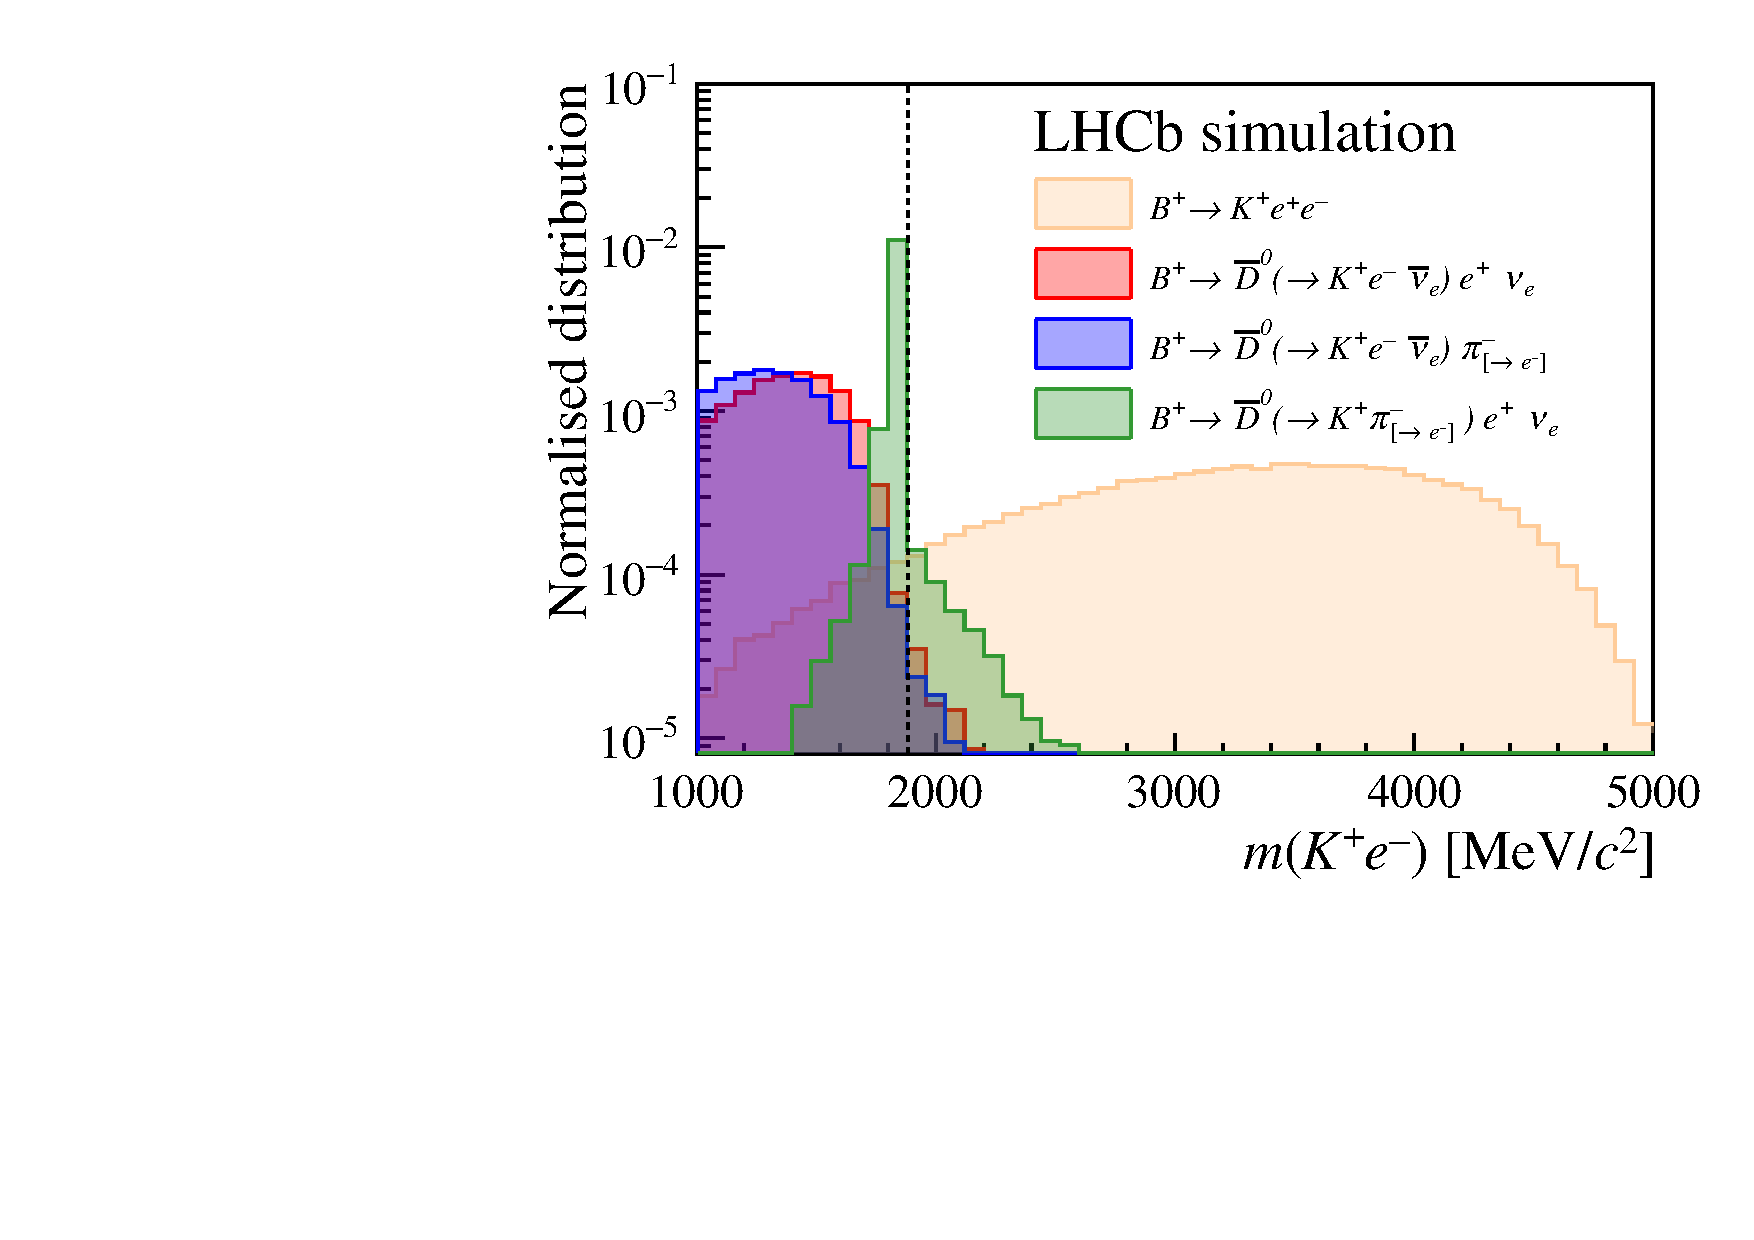
\includegraphics[width=0.48\linewidth]{figures/Fig5a.pdf}
      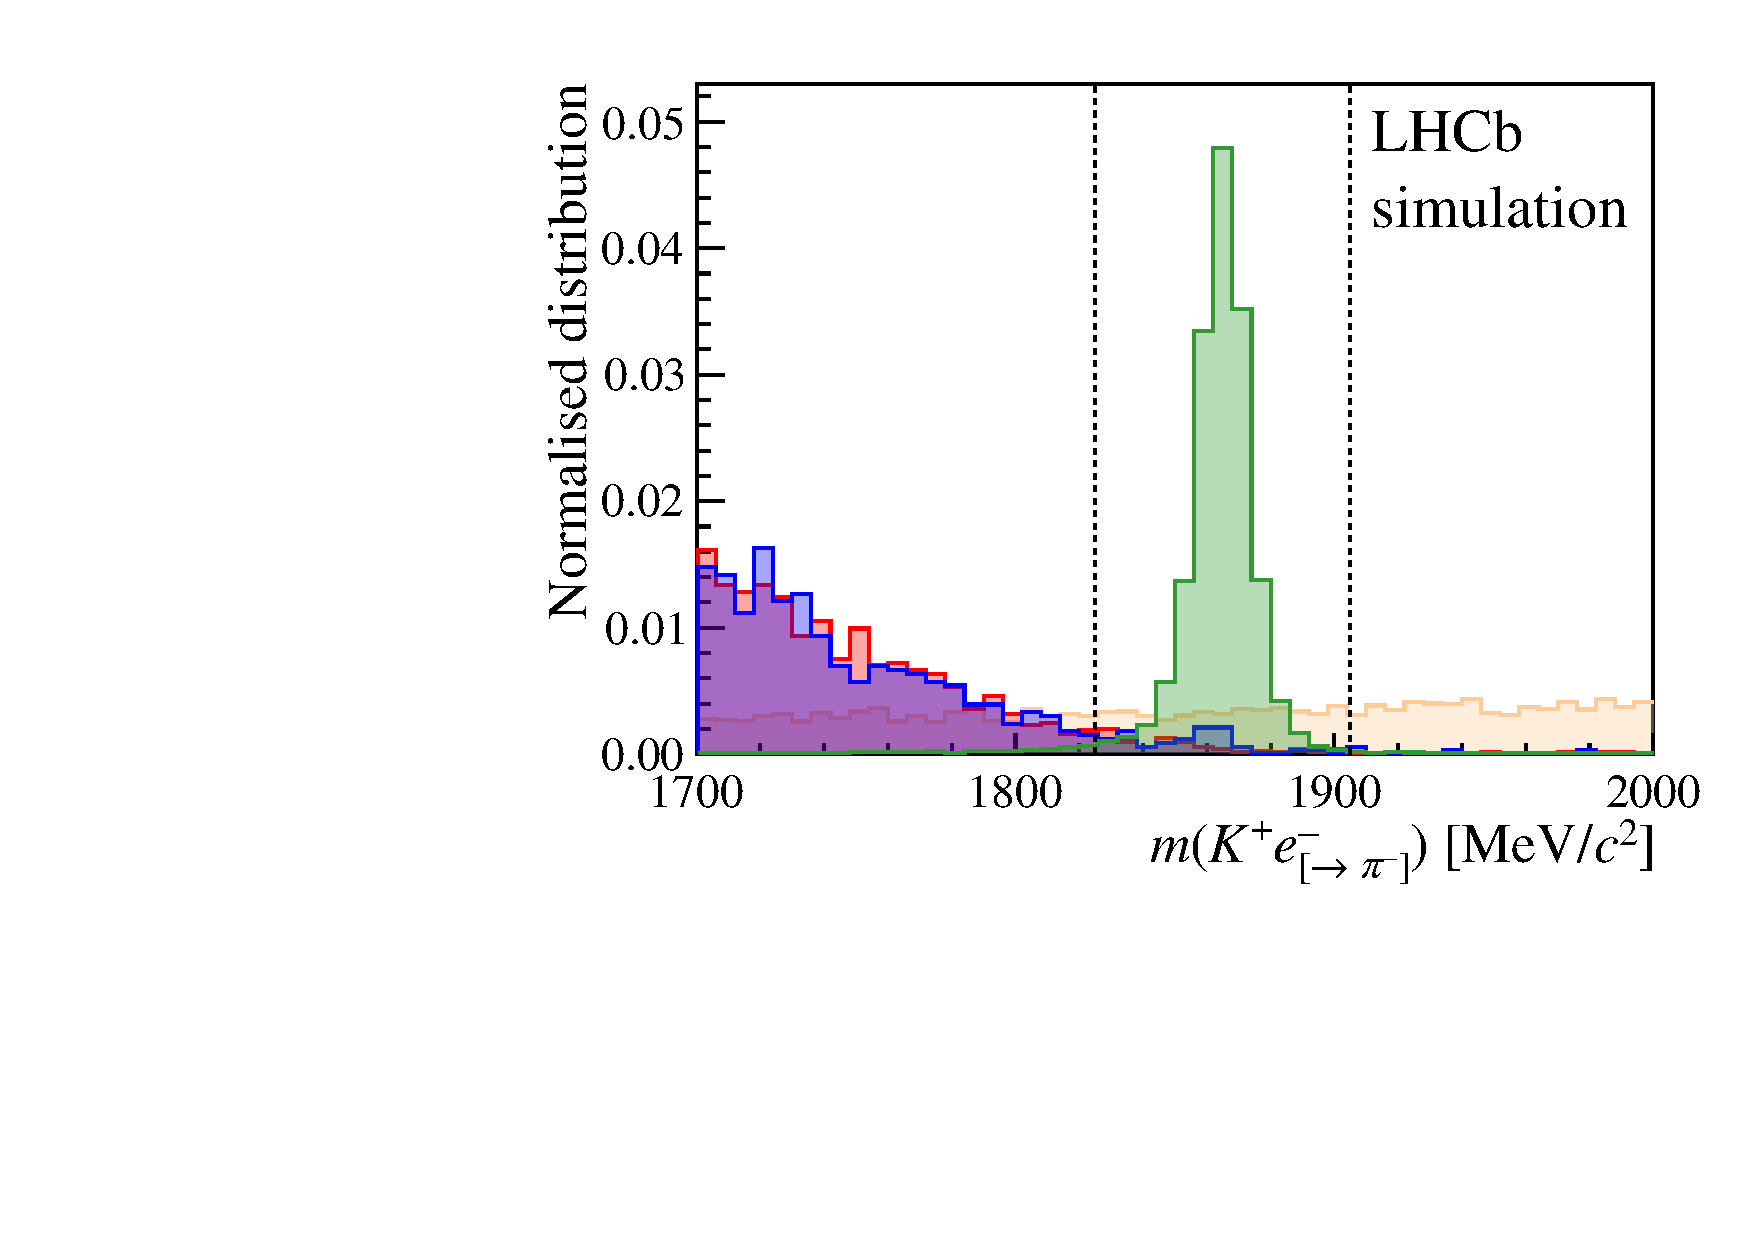
\includegraphics[width=0.48\linewidth]{figures/Fig5b.pdf}
   \end{center}
    \vspace*{-0.5cm}
   \caption{Simulated $K^+e^-$ mass distributions for  signal and various cascade background samples. The distributions are all normalised to unity.  (Left, with log $y$-scale)
   the bremsstrahlung correction to the momentum of the electron is applied, resulting in a tail to the right. The region to the left of the vertical dashed line is rejected. (Right, with linear $y$-scale) the mass is computed only from the track information. The notation $\pi^-_{[\rightarrow e^-]}$ ($e^-_{[\rightarrow \pi^-]}$) is used to denote an electron (pion) that is misidentified as a pion (electron). The region between the dashed vertical lines is rejected. }\label{fig:cascadeVeto}
\end{figure}

Background from other exclusive $B$-hadron decays requires at least two particles to be misidentified. These include the decays \BuKpipi, and misreconstructed \BuJpsiKll and \BuPsiKll decays. In the latter two decays the kaon is misidentified as a lepton and the lepton (of the same electric charge) as a kaon. Such background is reduced to a negligible level by particle-identification criteria. Background from decays with a photon converted into an \epem pair are also negligible due to the \qsq selection.


\subsubsection*{Multivariate selection}

A Boosted Decision Tree (BDT)  algorithm~\cite{Breiman} with gradient boosting~\cite{GradBoost} is used to reduce combinatorial background. For the nonresonant muon mode and for each of the three different trigger categories of the 
nonresonant electron mode, a single BDT classifier is trained for the 7 and $8\tev$ data, and an additional classifier is trained for the $13\tev$ data. The BDT output is not strongly correlated with \qsq and the same classifiers are used to select the respective resonant decays. 
In order to train the classifier, simulated nonresonant \BuKll decays are used as a proxy for the signal and nonresonant \Kll candidates selected from the data with $\mKll > 5.4\gevcc$ are used as a background sample. The $k$-folding technique is used in the training and testing~\cite{Blum:1999:BHB:307400.307439}. 
The classifier includes the following variables:  the  \pt of the \Bp, \Kp and dilepton candidates, and the minimum and maximum \pt of the leptons;  the \Bp, dilepton and \Kp \chisqip with respect to the associated PV, where \chisqip is defined as the difference in the vertex-fit \chisq of the PV reconstructed with and without the considered particle; the minimum and maximum \chisqip of the leptons; the \Bp vertex-fit quality; the statistical significance of the \Bp flight distance; and the angle between the \Bp candidate momentum vector and the direction between the associated PV and the \Bp decay vertex. 
For each of the classifiers, a requirement is placed on the output variable in order to maximise the predicted significance of the nonresonant signal yield. For the electron modes that dictate the \RK precision, this requirement reduces the combinatorial background by approximately $99\%$, while retaining $85\%$ of the signal mode. The muon BDT classifier has similar performance. In both cases the efficiency of the BDT selection has negligible dependence on \mKll in the regions used to determine the event yields. 

\subsubsection*{Calibration of simulation} 

The simulated data used in this analysis are produced using the software described in Refs.~\cite{Sjostrand:2006za,*Sjostrand:2007gs,LHCb-PROC-2010-056,Lange:2001uf,Allison:2006ve, *Agostinelli:2002hh,LHCb-PROC-2011-006}. Bremsstrahlung emission in the decay of particles is simulated using the \photosplusplus software in the default configuration~\cite{ Davidson:2010ew}, which is observed to agree with a full quantum electrodynamics calculation at the level of $1\%$~\cite{Bordone:2016gaq}.

Simulated events are weighted to correct for the imperfect modelling using control channels. The \Bu production kinematics are corrected using \BuJpsiKll events. The particle-identification performance is calibrated using data, where the species of particles in the final state can be unambiguously determined purely on the basis of the kinematics. 
The calibration samples consist of $\decay{\Dstarp}{\Dz(\to\Km\pip)\pip}$, $\decay{\jpsi}{\mumu}$, and \BuJpsiKee decays, from which kaons, muons, and electrons, respectively, can be selected without applying particle-identification requirements. The performance of the particle-identification requirements is then evaluated from the proportion of events in these samples which fulfil the particle-identification selection criteria. The trigger response is corrected using weights applied to simulation as a function of variables relevant to the trigger algorithms. The weights are calculated by requiring that simulated \BuJpsiKll events  exhibit the same trigger performance as the control data. The \BuJpsiKll events selected from the data have also been used to demonstrate control of the electron track-reconstruction efficiency at the percent level~\cite{Aaij:2019vvl}.
Whenever \BuJpsiKll events are used to correct the simulation, the correlations between calibration and measurement samples are taken into account in the results and cross-checks presented in the article. 

\subsubsection*{Likelihood fit} 

An unbinned extended maximum-likelihood fit is made to the \mKee and \mKmm distributions of nonresonant candidates. The value of \RK is a fit parameter, which is related to the signal yields and efficiencies according to,  
\begin{eqnarray}
    \label{eq:RKdetail}
       \RK &=&\frac{N(\BuKmm)}{\varepsilon(\BuKmm)}\cdot\frac{\varepsilon(\BuKee)}{N(\BuKee)} \times \nonumber\\
 & & \frac{\varepsilon(\BuJpsiKmm)}{N(\BuJpsiKmm)}\cdot\frac{N(\BuJpsiKee)}{\varepsilon(\BuJpsiKee)} \,, 
\end{eqnarray}
\noindent where $N(X)$  indicates the  yield  of  decay  mode $X$,  which  is  obtained from a fit to the invariant mass \mKll (or \mKllconst) with a suitable requirement on \qsq, and $\varepsilon(X)$ is the efficiency for selecting decay mode $X$. In order to take into account the correlation between the selection efficiencies, the \mKee and \mKmm distributions of nonresonant candidates in each of the different trigger categories and data-taking periods are fitted simultaneously. 

The mass-shape parameters are derived from the calibrated simulation. The four signal modes are modelled by multiple Gaussian functions with  power-law tails on both sides of the peak~\cite{Skwarnicki:1986xj,Santos:2013gra} although the differing detector response gives different shapes for the electron and muon modes. The signal mass shapes of the electron modes are described with the sum of three distributions, which model whether the ECAL energy deposit from a bremsstrahlung photon was added to both, either, or neither of the \epm candidates. The expected values from simulated events are used to constrain the fraction of signal decays in each of these categories.

Data are used to correct the simulated $K\pi$ mass spectrum for \BuBdKpiplusee and \BuBdKpijpsi decays~\cite{LHCb-PAPER-2016-025}. The calibrated simulation is used subsequently to obtain the \mKll mass shape and relative fractions of these background components. In order to accommodate possible lepton-universality violation in these partially reconstructed processes, which are underpinned by the same $\bquarkbar\to\squarkbar$ quark-level transitions as those of interest, the overall yield of such decays is left to vary freely in the fit. The shape of the \BuJpsipi background contribution is taken from simulation but the size with respect to the \BuJpsiK mode is constrained using the known ratio of the relevant branching fractions~\cite{LHCb-PAPER-2016-051, PDG2020} and efficiencies.

In the fits to nonresonant \BuKee candidates, the mass shape of the background from \BuJpsiKee decays with an emitted photon that is not reconstructed is also taken from simulation and, adjusting for the relevant selection efficiency, its yield is constrained to the value from the fit to the resonant mode within its uncertainty.   
In all fits, the combinatorial background is modelled with an exponential function with a freely varying yield and shape.

The fits to the nonresonant (resonant) decay modes in different data-taking periods and trigger categories are shown in Fig.~\ref{fig:nonresfits_categories}  (Fig.~\ref{fig:resfits_categories}).
For the resonant modes the results from independent fits to each period/category are shown. Conversely, the nonresonant distributions show the projections from the simultaneous fit across data taking periods and trigger categories that is used to obtain \RK. The fitted yields for the resonant and nonresonant decays are given in Table~\ref{tab:yields}. 

\begin{table}[b]
\centering
\caption{Yields of the  nonresonant and resonant decay modes obtained from the fits to the data.} \label{tab:yields}
\begin{tabular}{lc}
\toprule
Decay mode  &   Yield             \\
\midrule
\BuKee      &   $\phantom{0\,00}1\,640 \pm \phantom{0\,0}70$ \\
\BuKmm      &   $\phantom{0\,00}3\,850 \pm \phantom{0\,0}70$ \\
\BuJpsiKee  &   $\phantom{0\,}743\,300 \pm \phantom{0\,}900$ \\
\BuJpsiKmm  &   $2\,288\,500 \pm 1\,500$      \\
\bottomrule
\end{tabular}
\end{table}


\begin{figure}
    \centering
    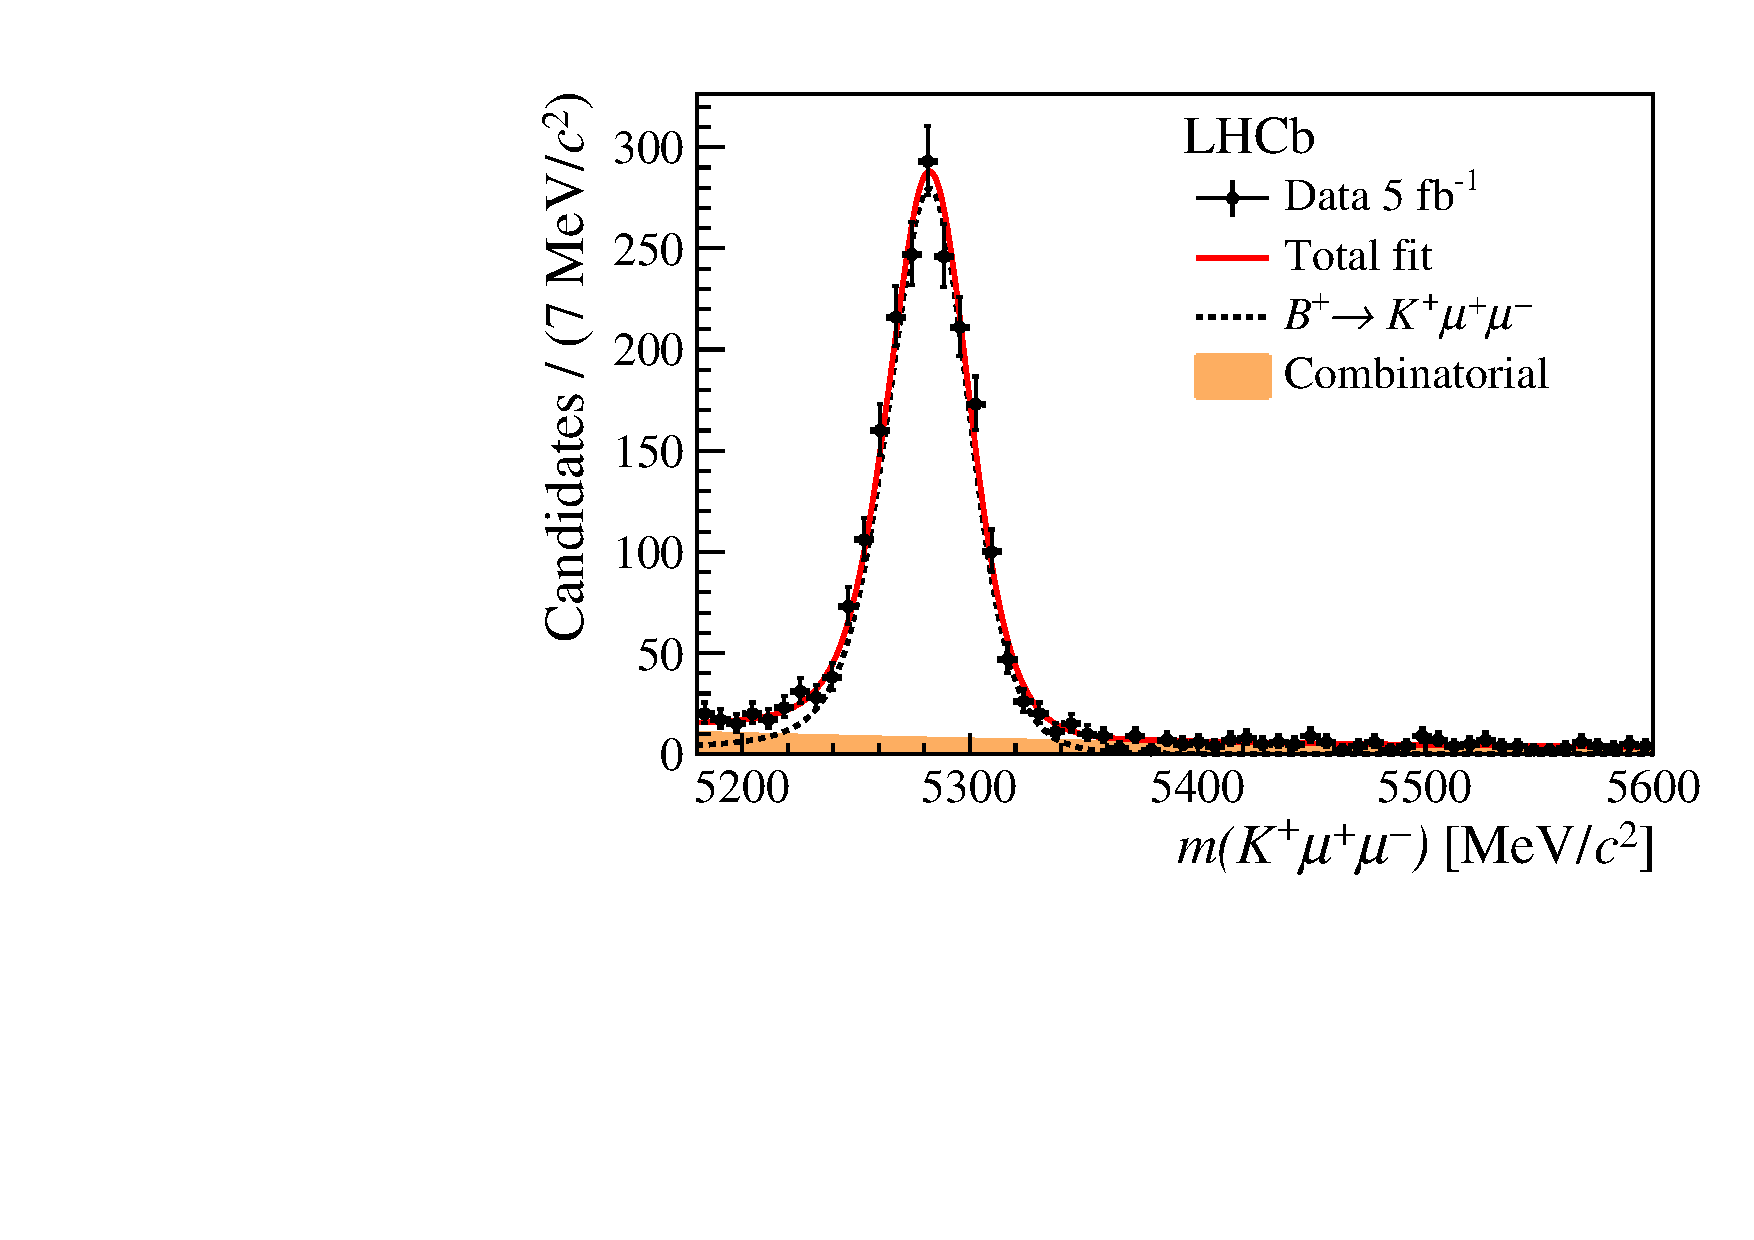
\includegraphics[width=0.45\textwidth]{figures/Fig6a.pdf}
    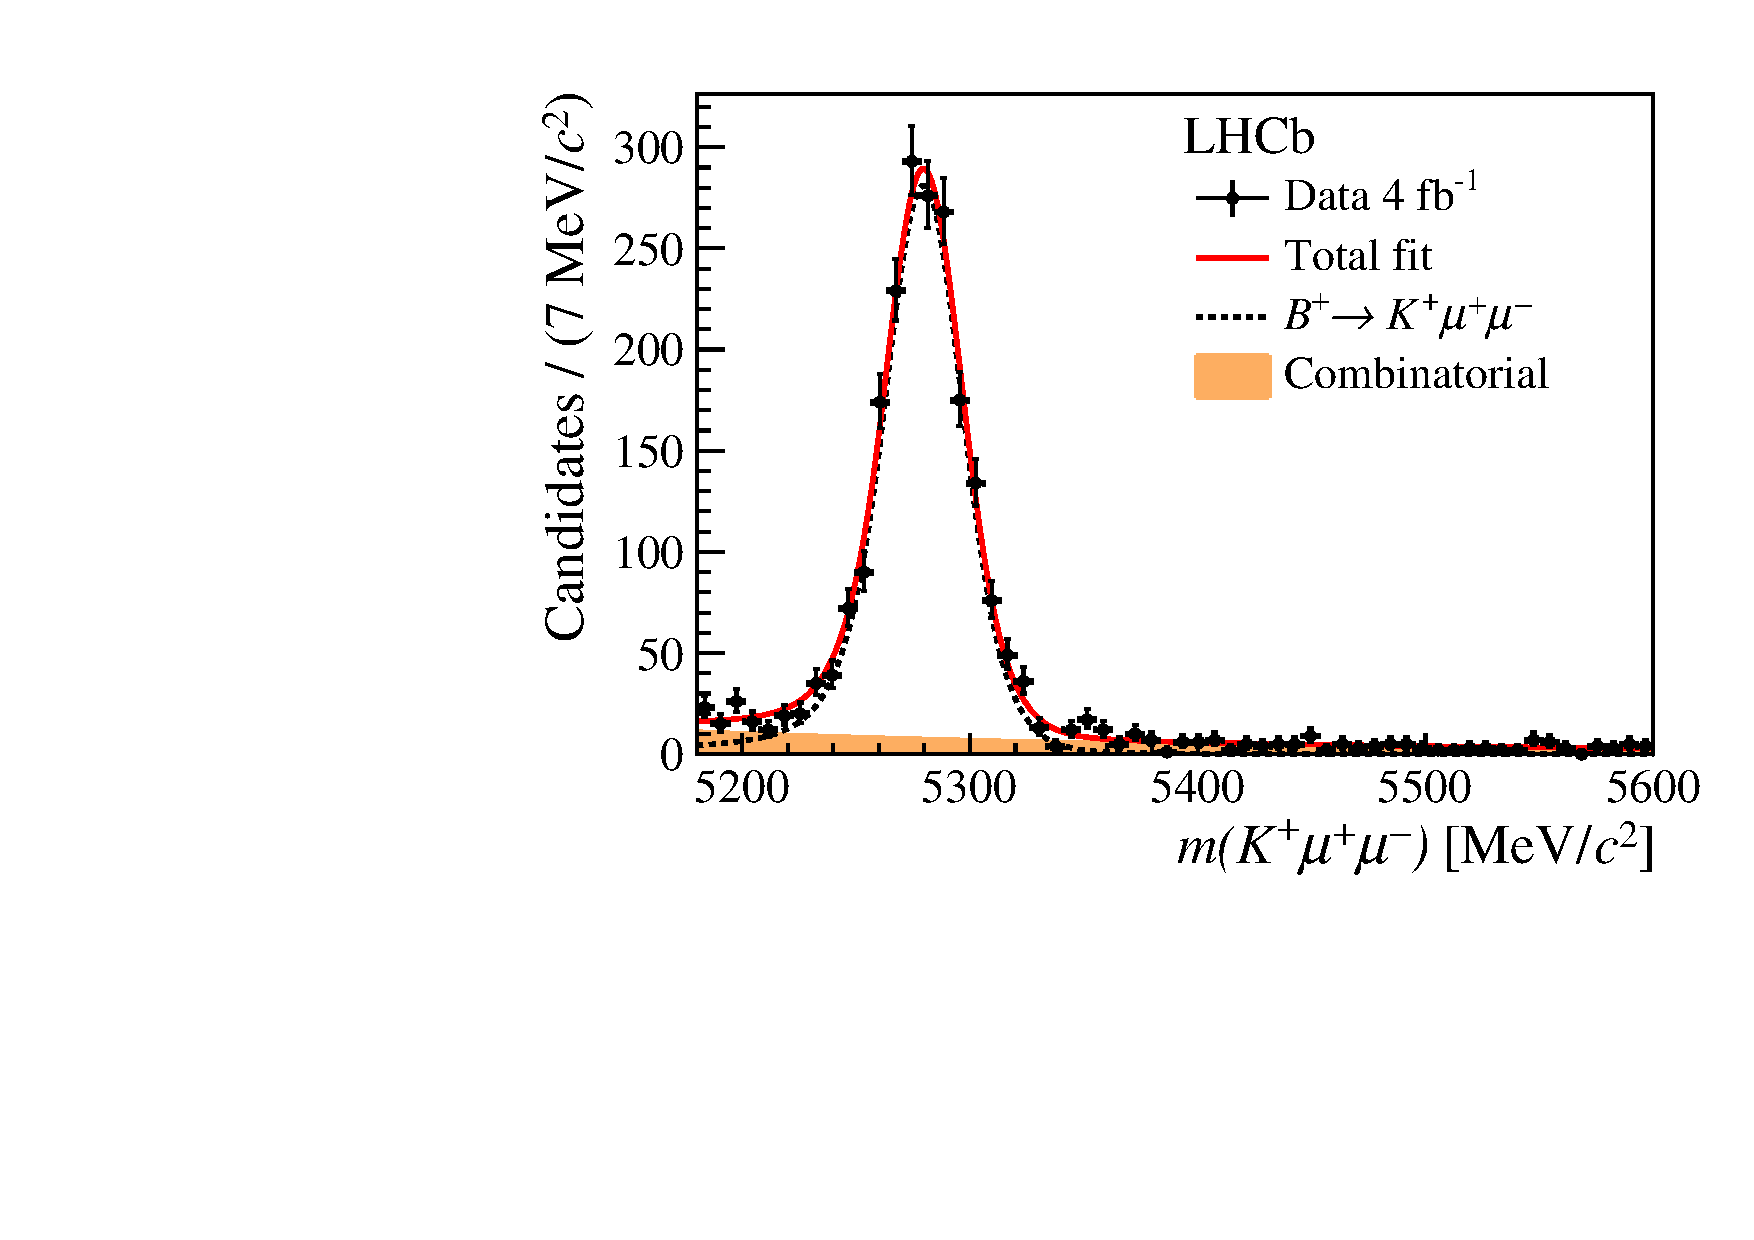
\includegraphics[width=0.45\textwidth]{figures/Fig6b.pdf}

    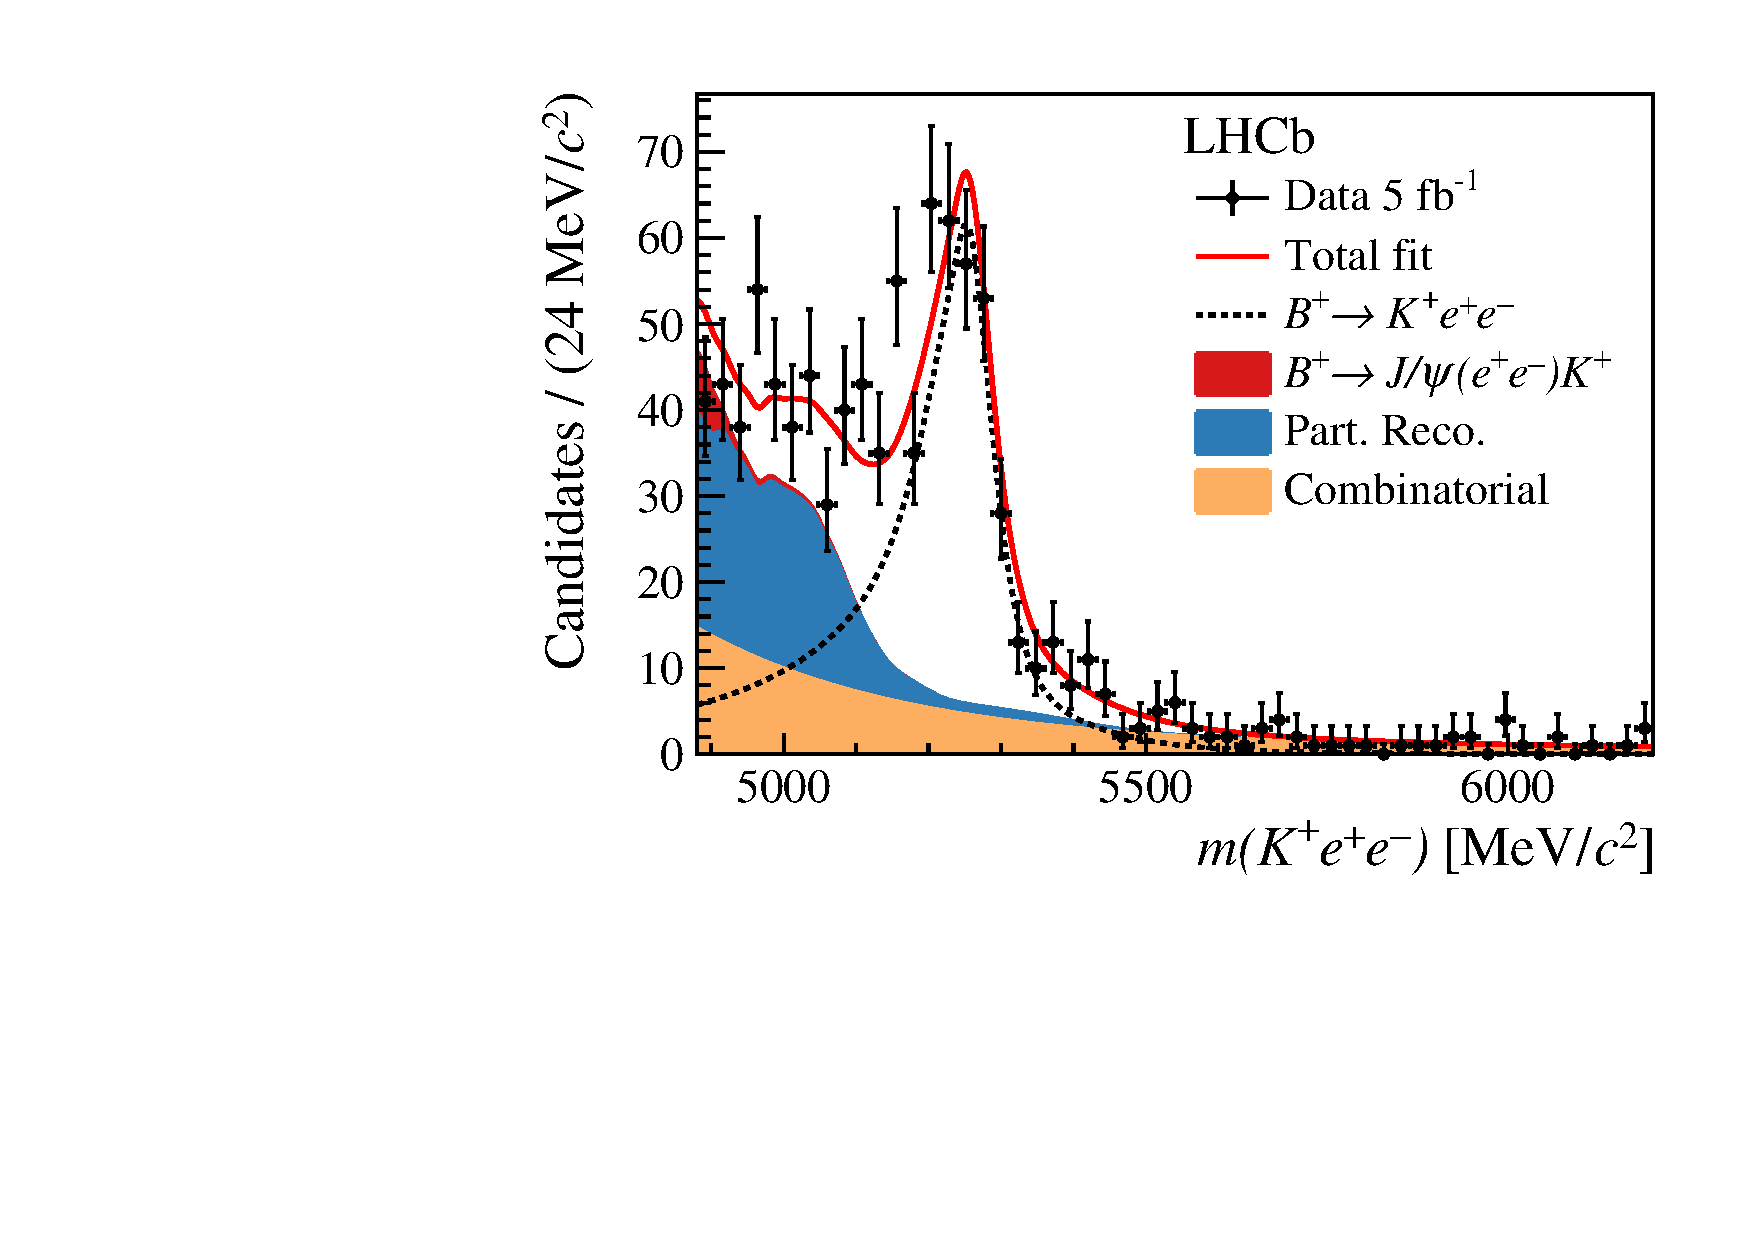
\includegraphics[width=0.45\textwidth]{figures/Fig6c.pdf}
    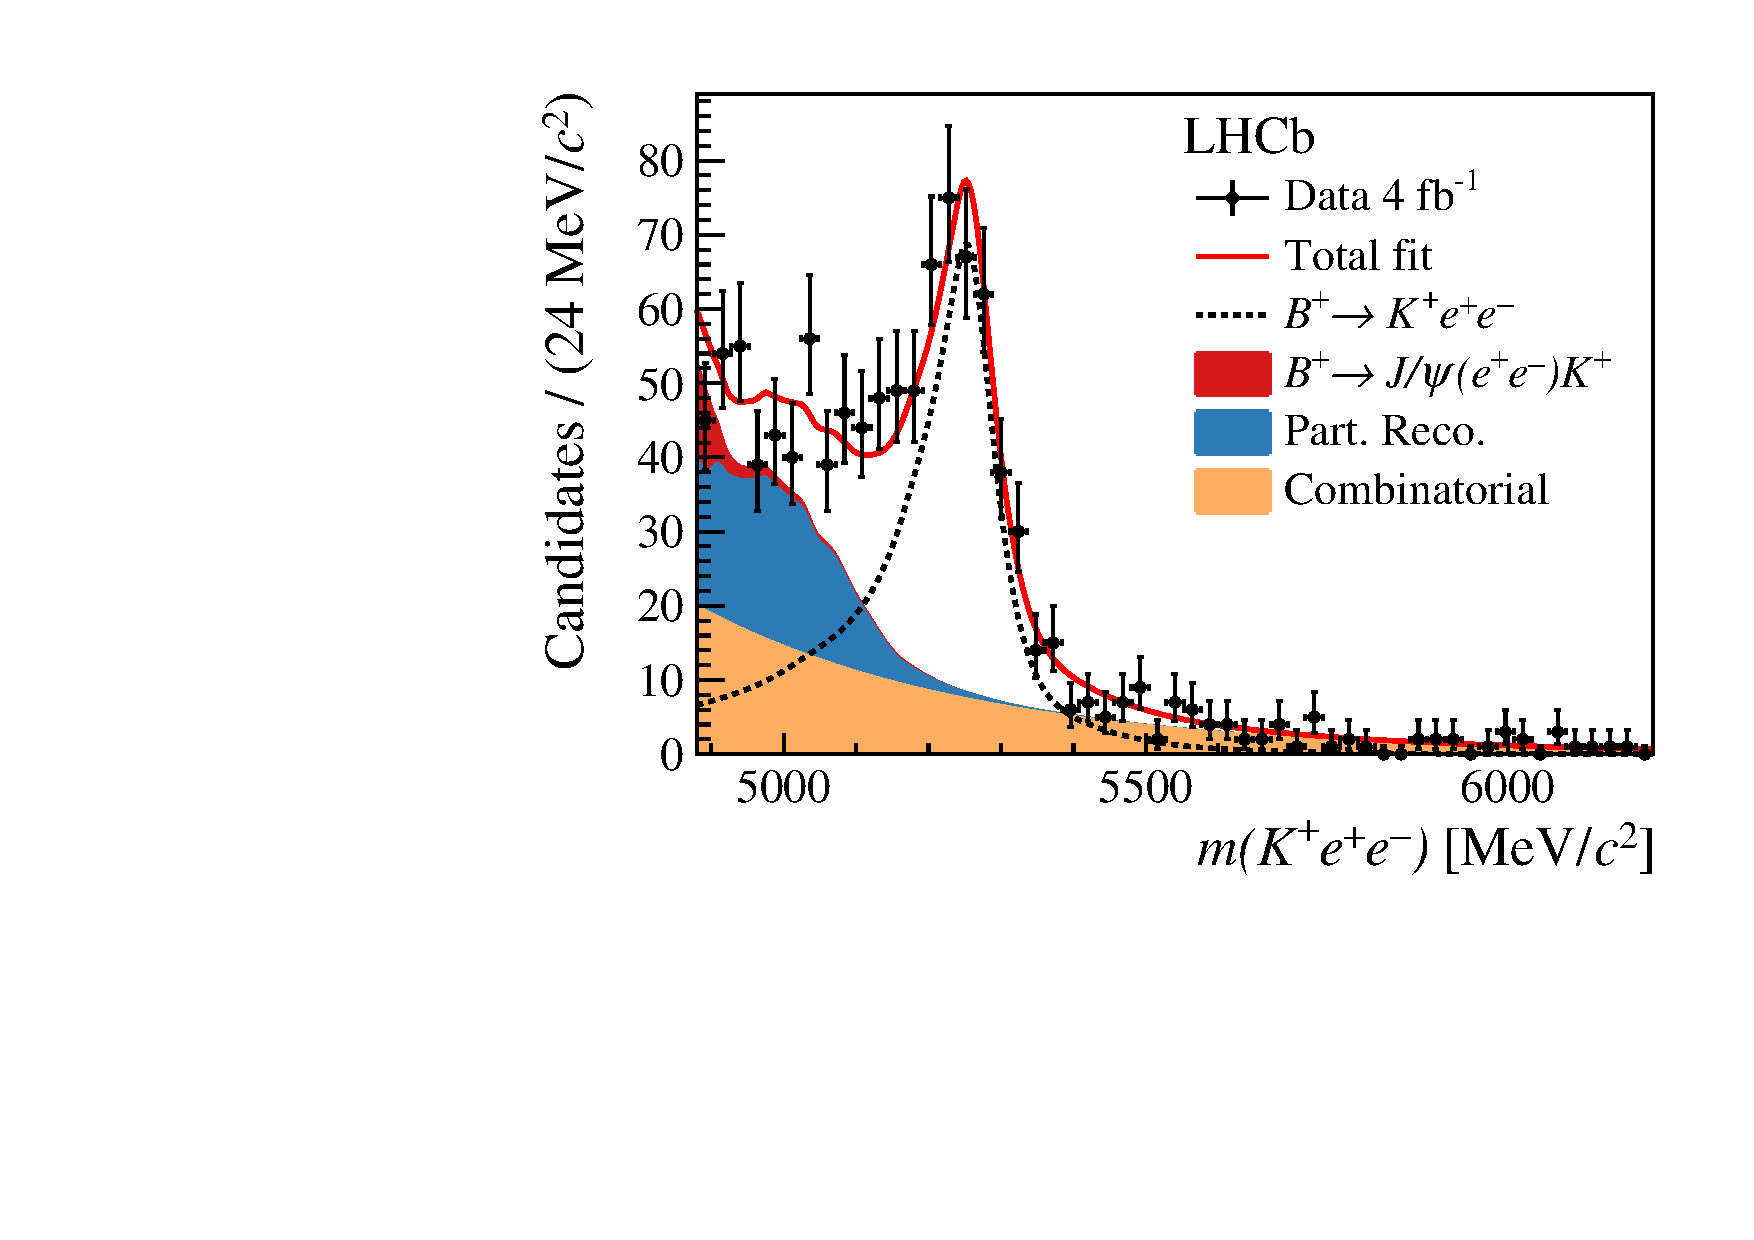
\includegraphics[width=0.45\textwidth]{figures/Fig6d.pdf}
    
    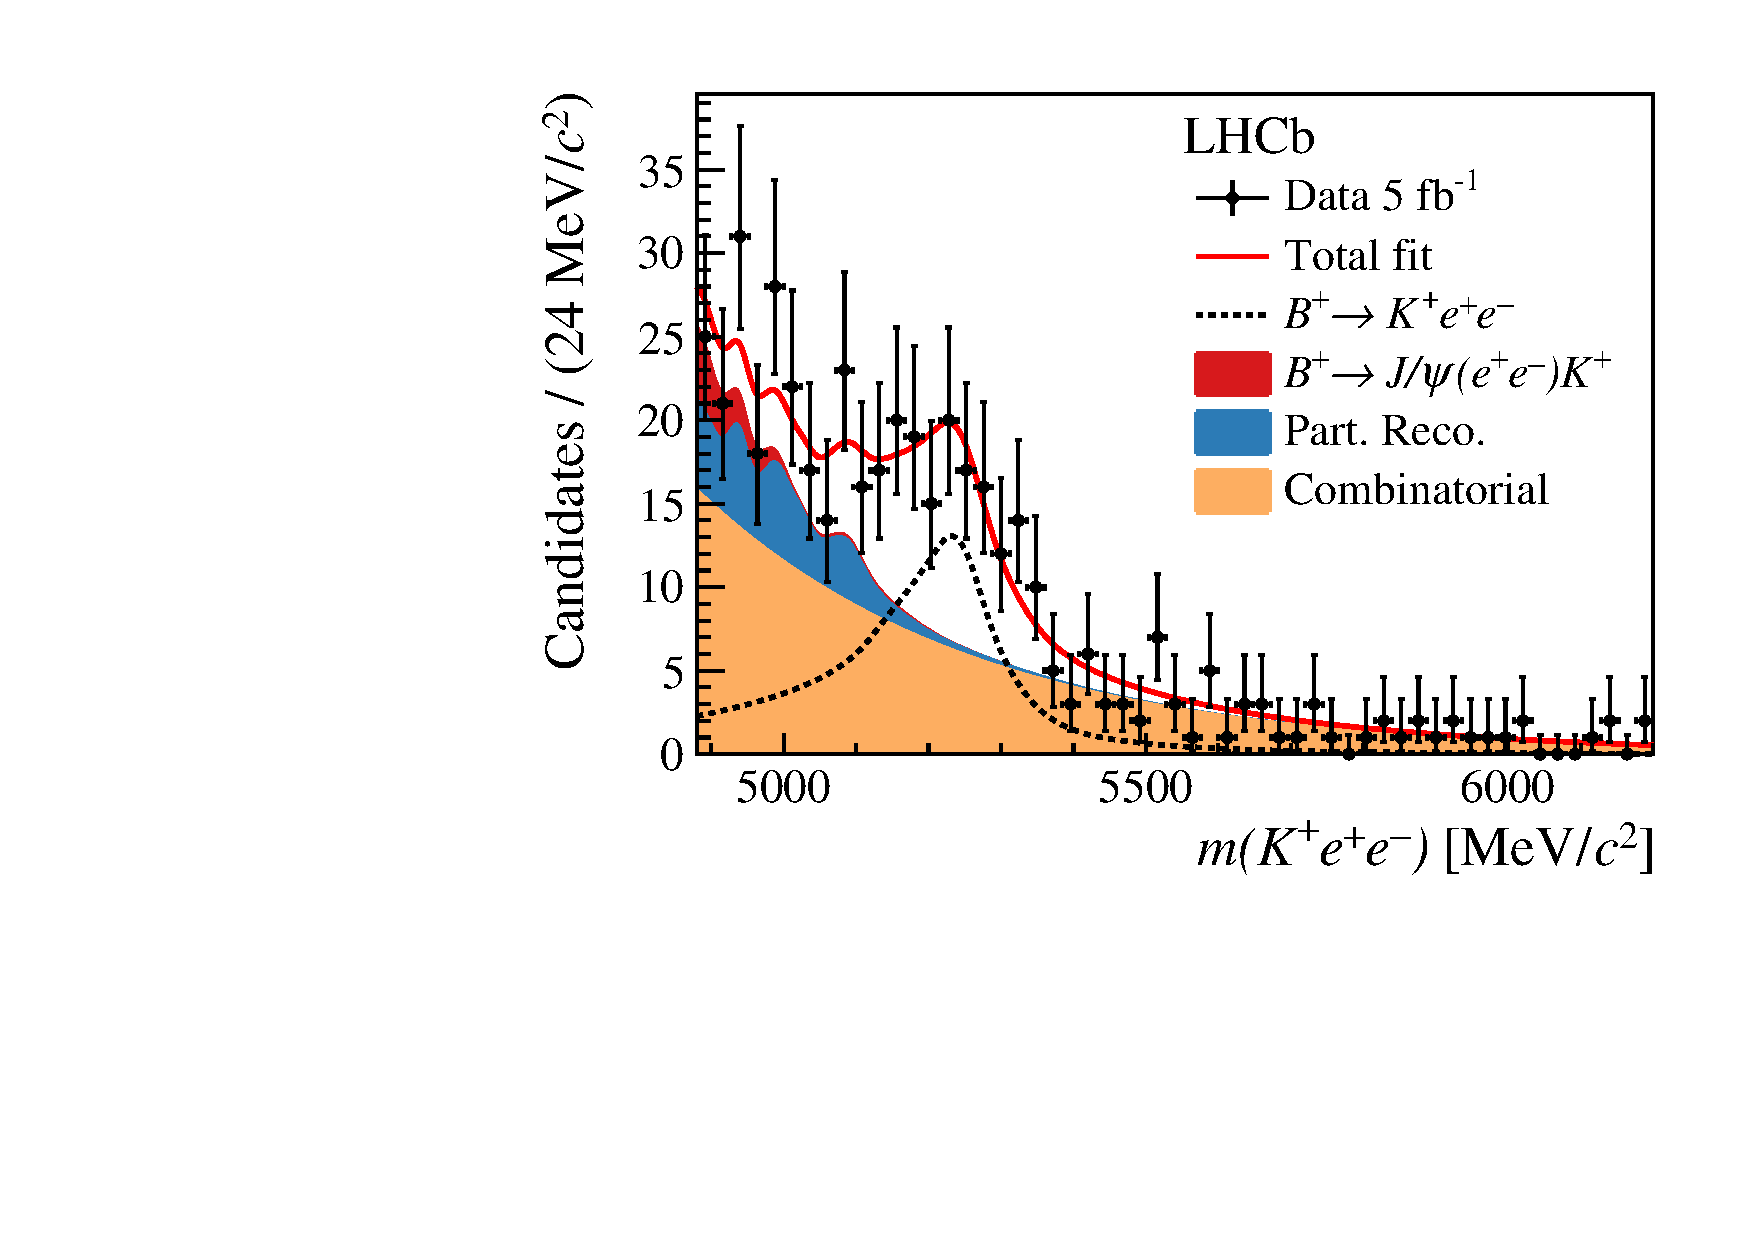
\includegraphics[width=0.45\textwidth]{figures/Fig6e.pdf}
    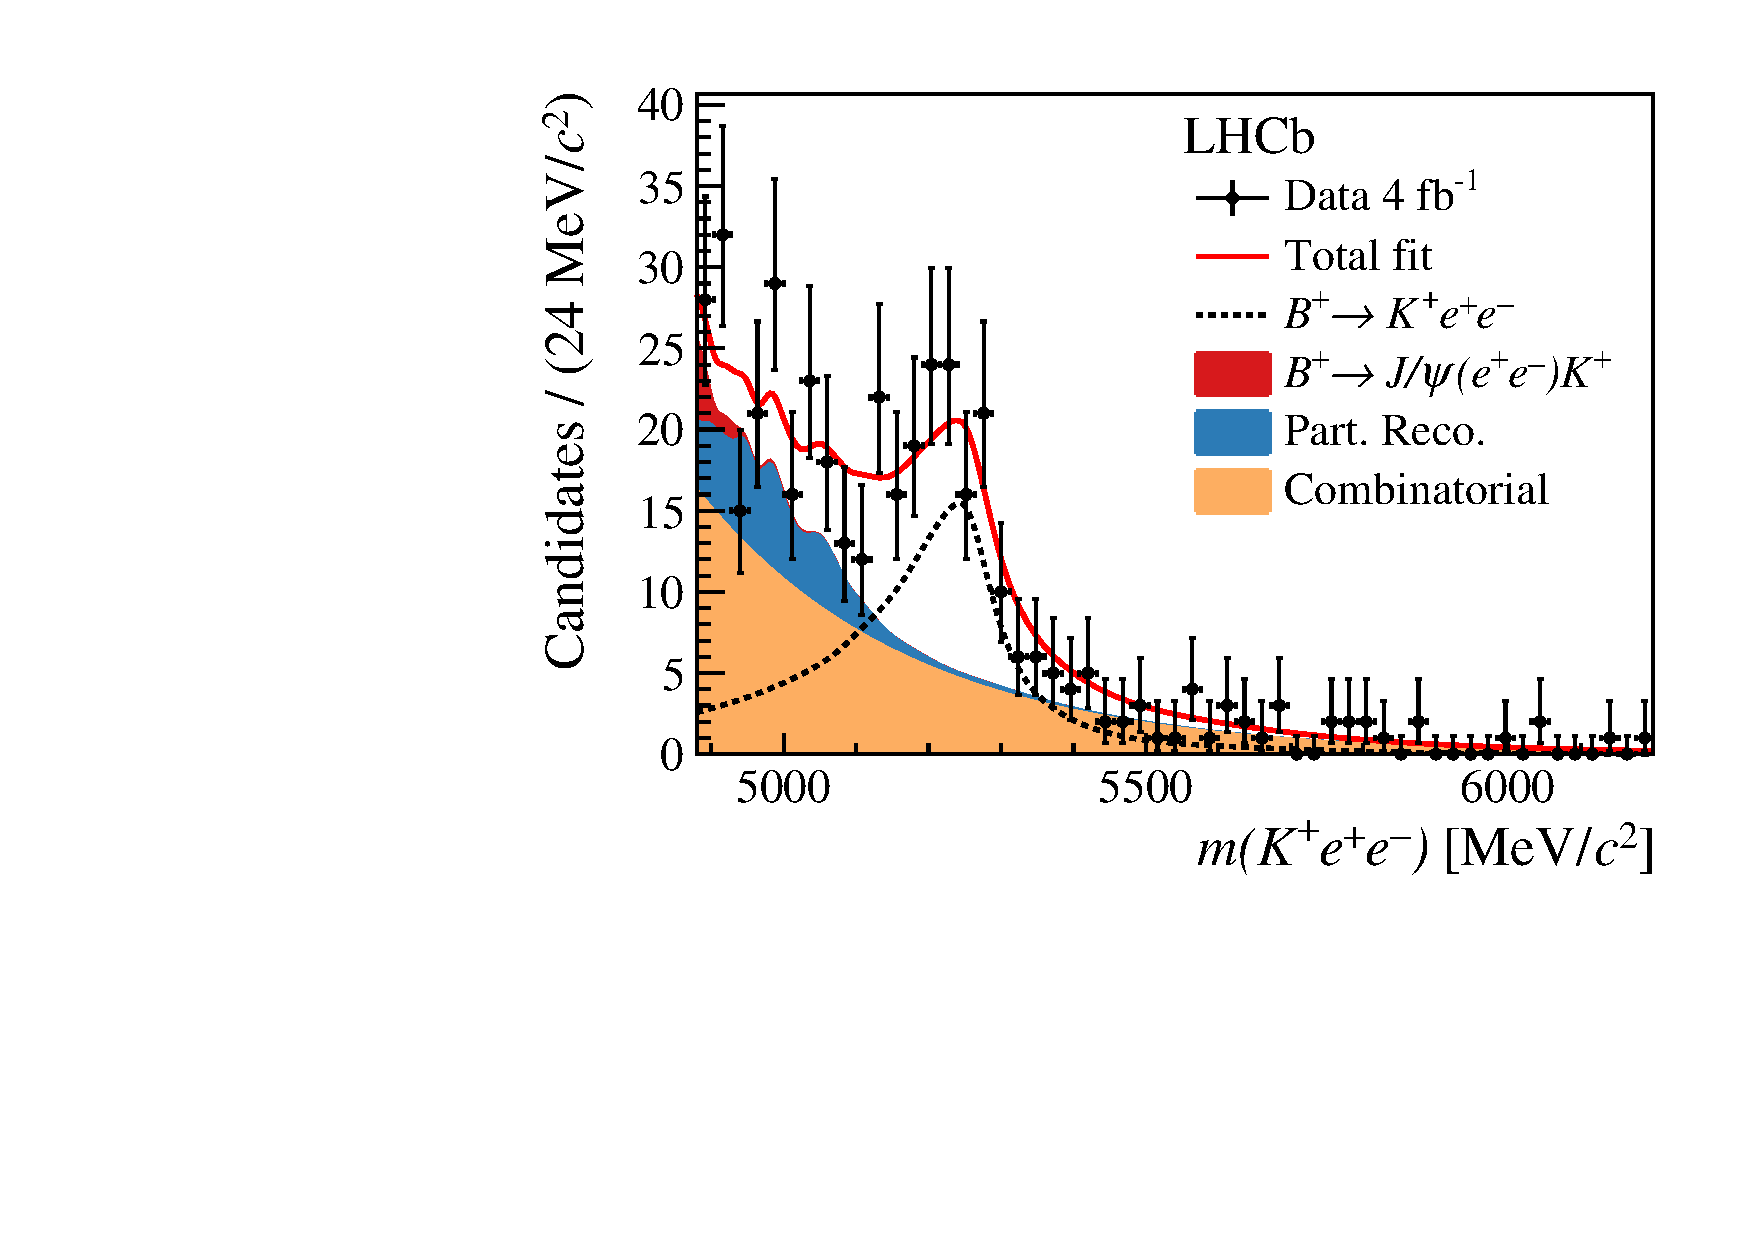
\includegraphics[width=0.45\textwidth]{figures/Fig6f.pdf}
    
    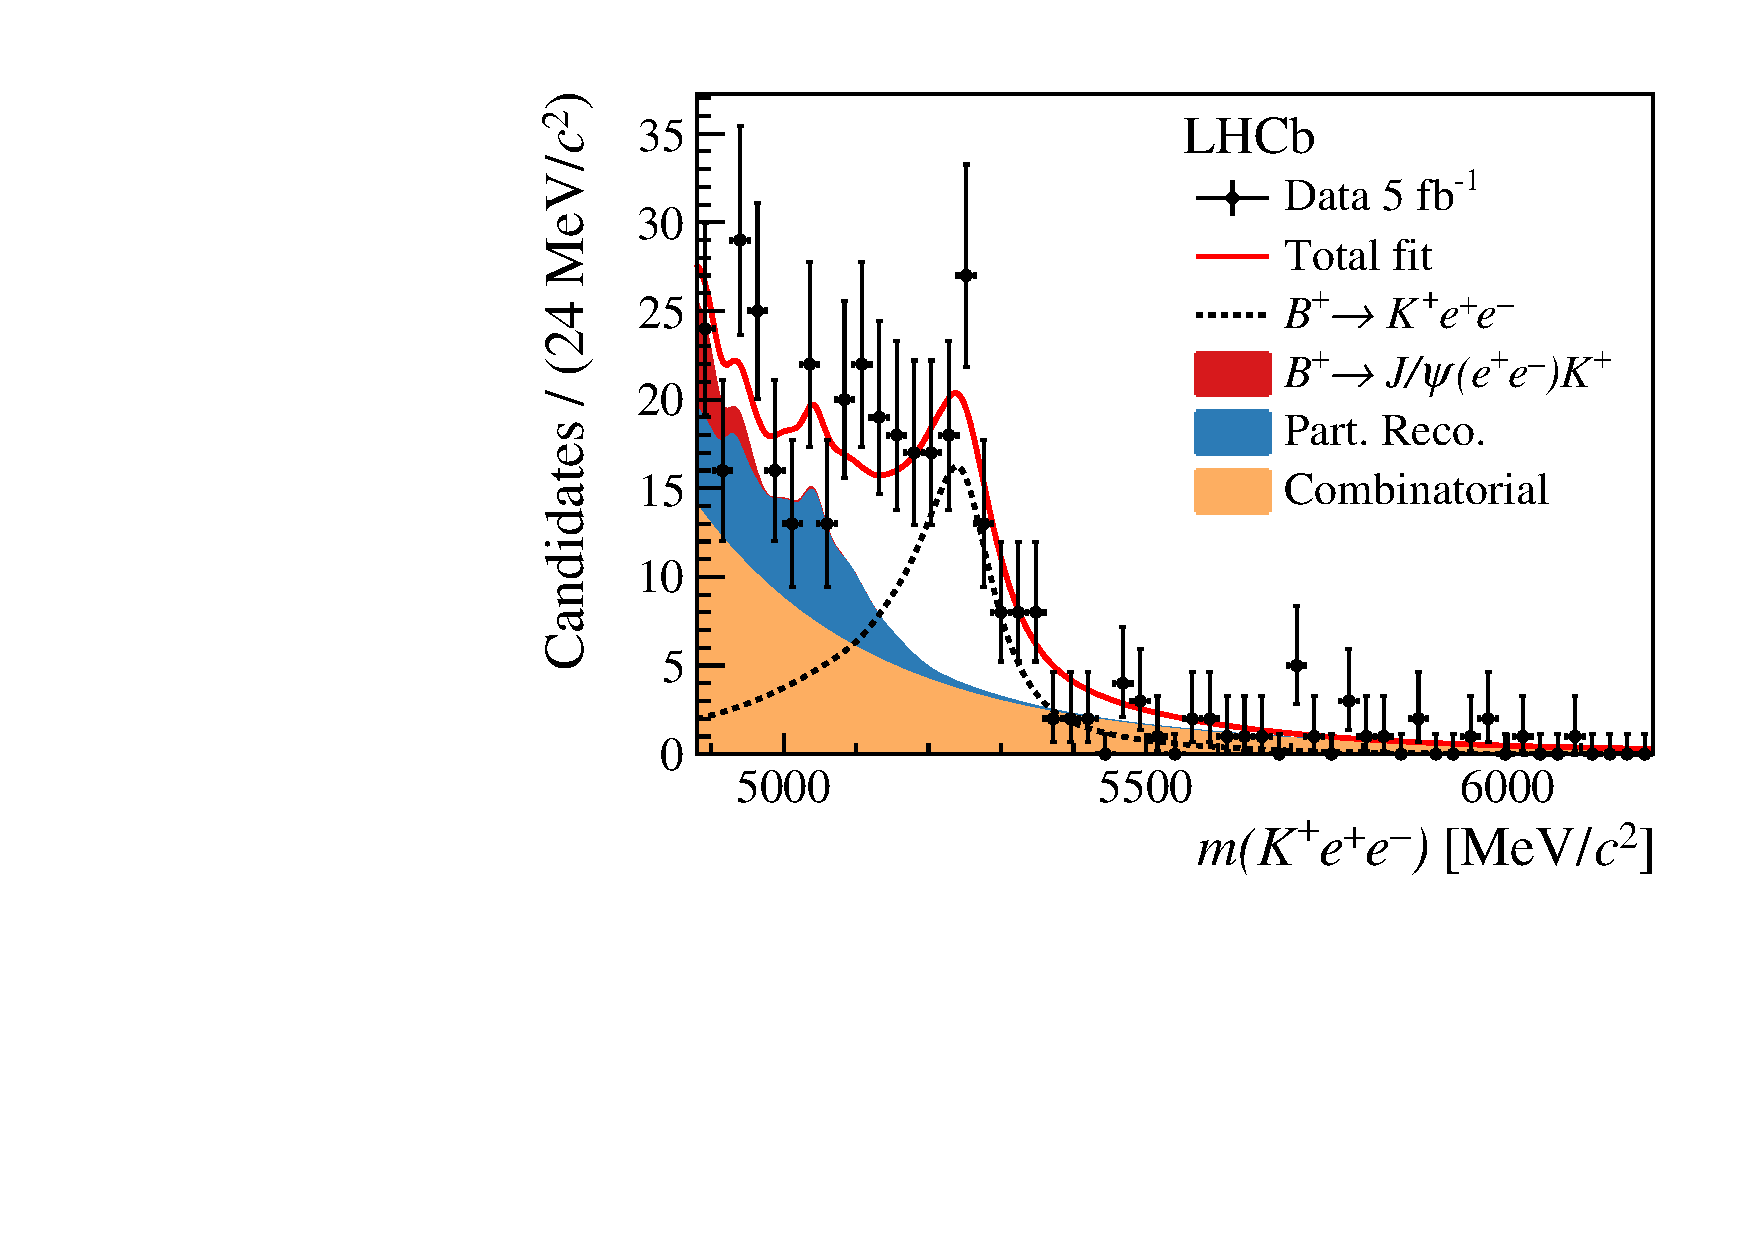
\includegraphics[width=0.45\textwidth]{figures/Fig6g.pdf}
    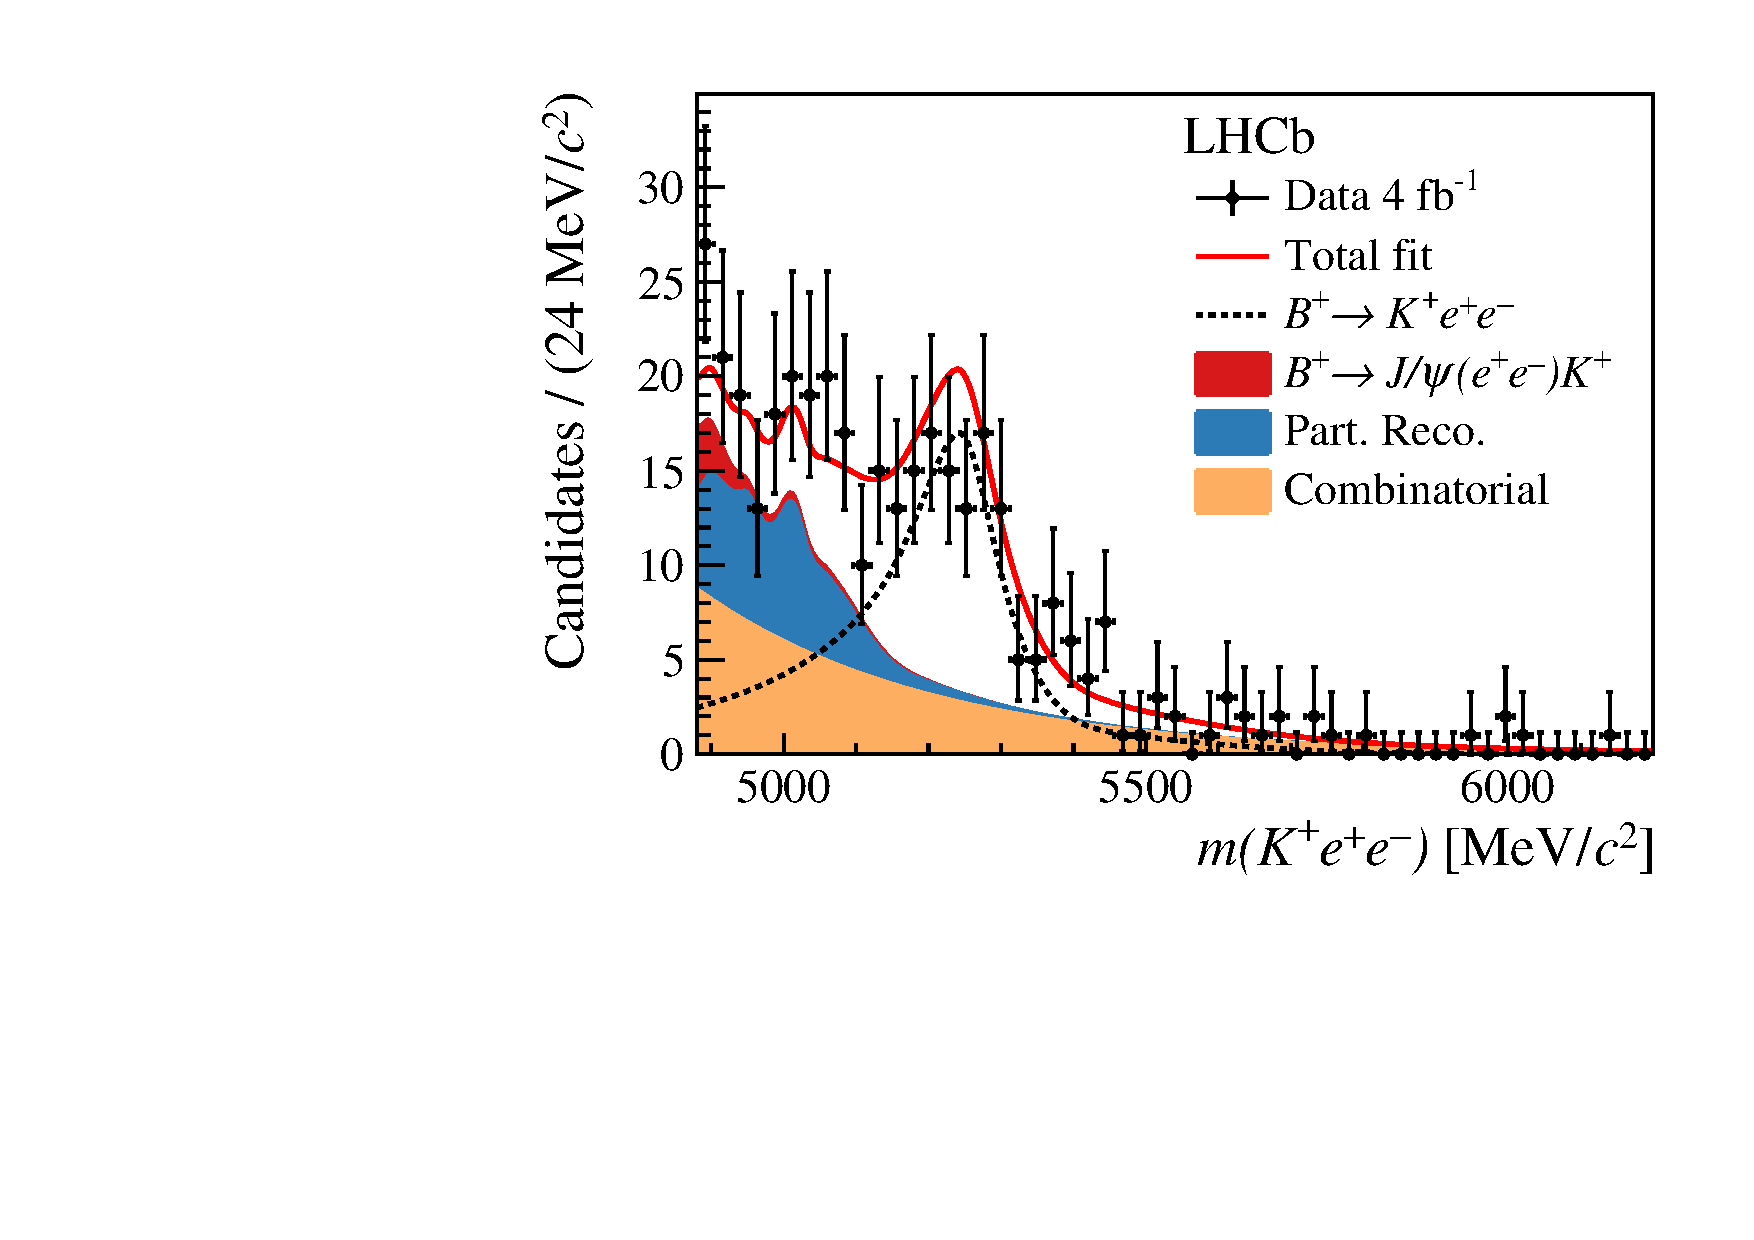
\includegraphics[width=0.45\textwidth]{figures/Fig6h.pdf}
    \caption{Candidate invariant mass distributions. Distribution of the invariant mass \mKll for nonresonant candidates in the (left) sample previously analysed~\cite{LHCb-PAPER-2019-009} and (right) the new data sample. The top row shows the fit to the muon modes and the subsequent rows the fits to the electron modes triggered by (second row) one of the electrons, (third row) the kaon and (last row) by other particles in the event. The fit projections are superimposed.
    }
    \label{fig:nonresfits_categories}
\end{figure}


\begin{figure}
    \centering
    % \includegraphics[width=0.45\textwidth]{figures/FigS5a.pdf}
    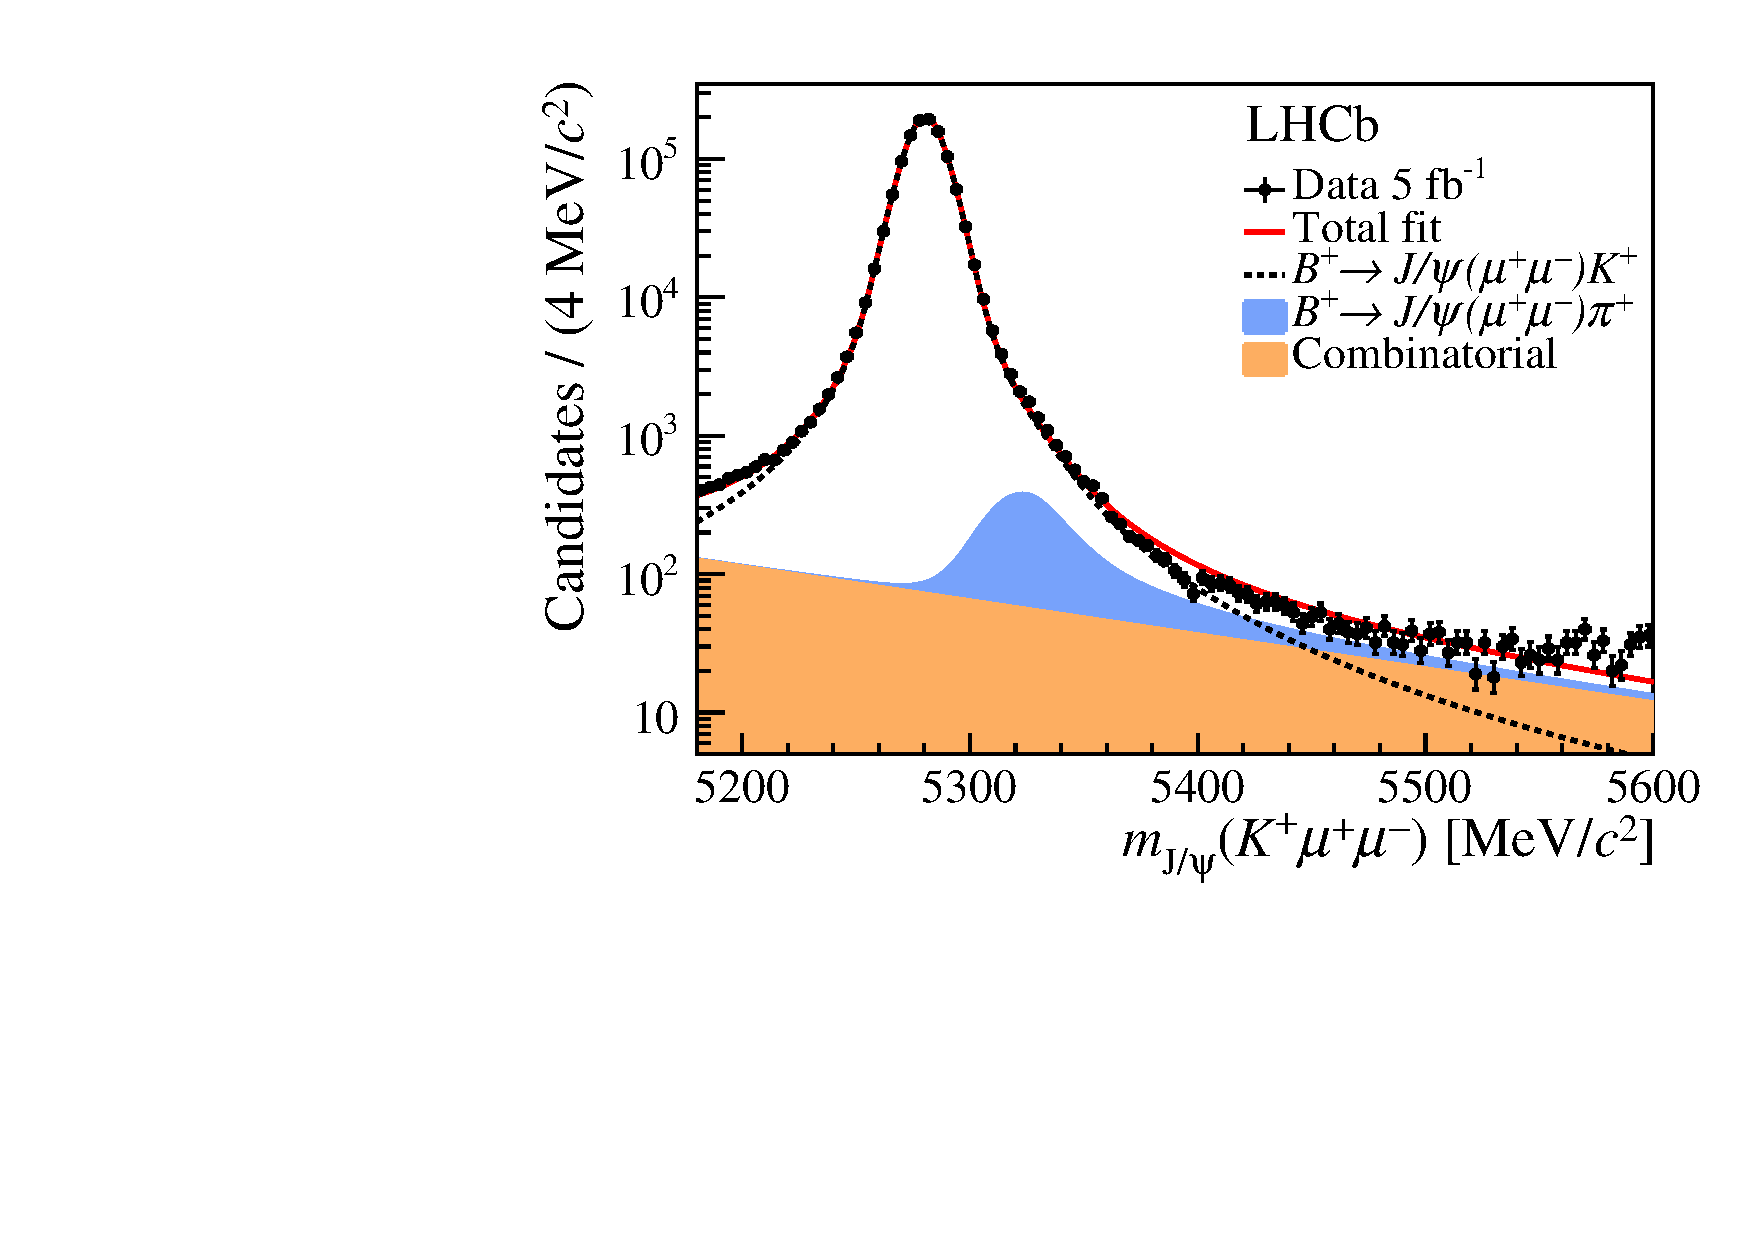
\includegraphics[width=0.45\textwidth]{figures/Fig7a.pdf}
    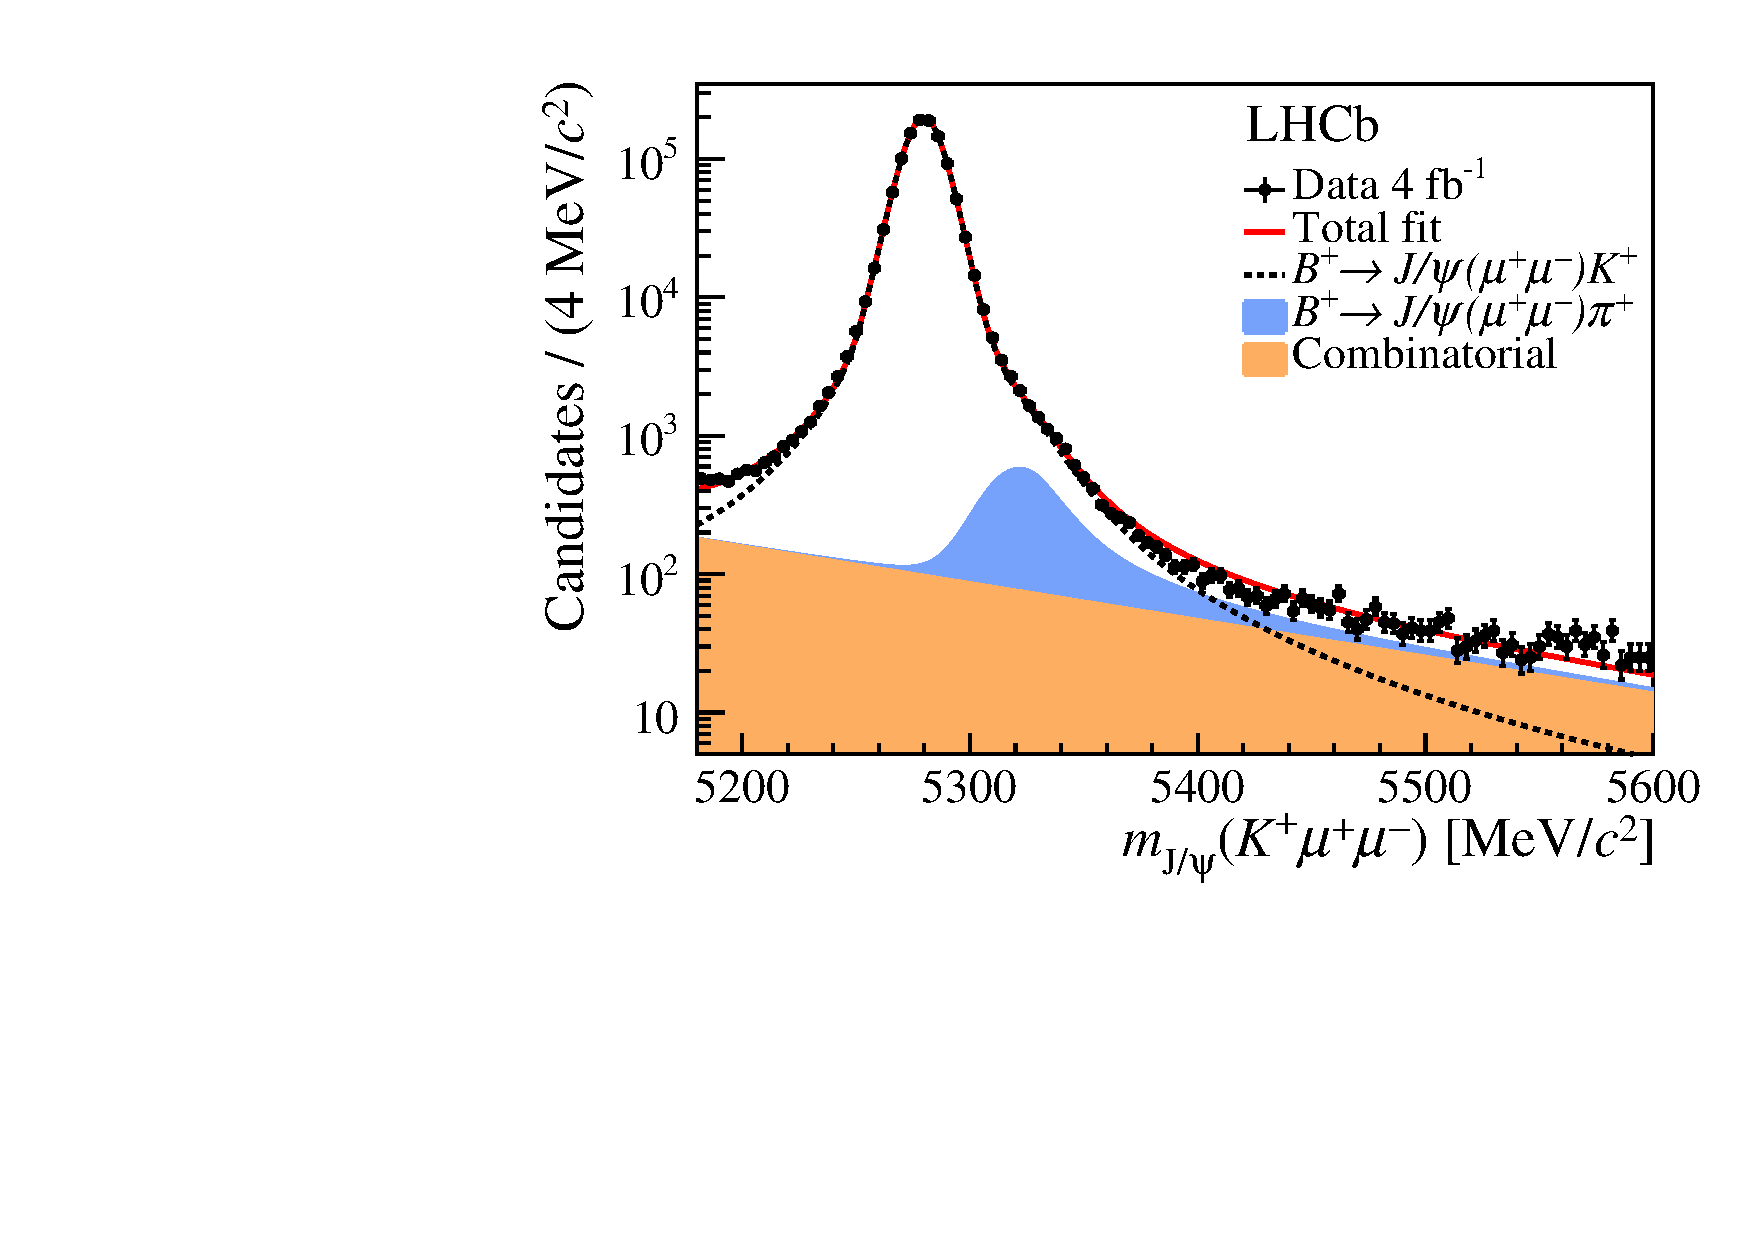
\includegraphics[width=0.45\textwidth]{figures/Fig7b.pdf}
    
    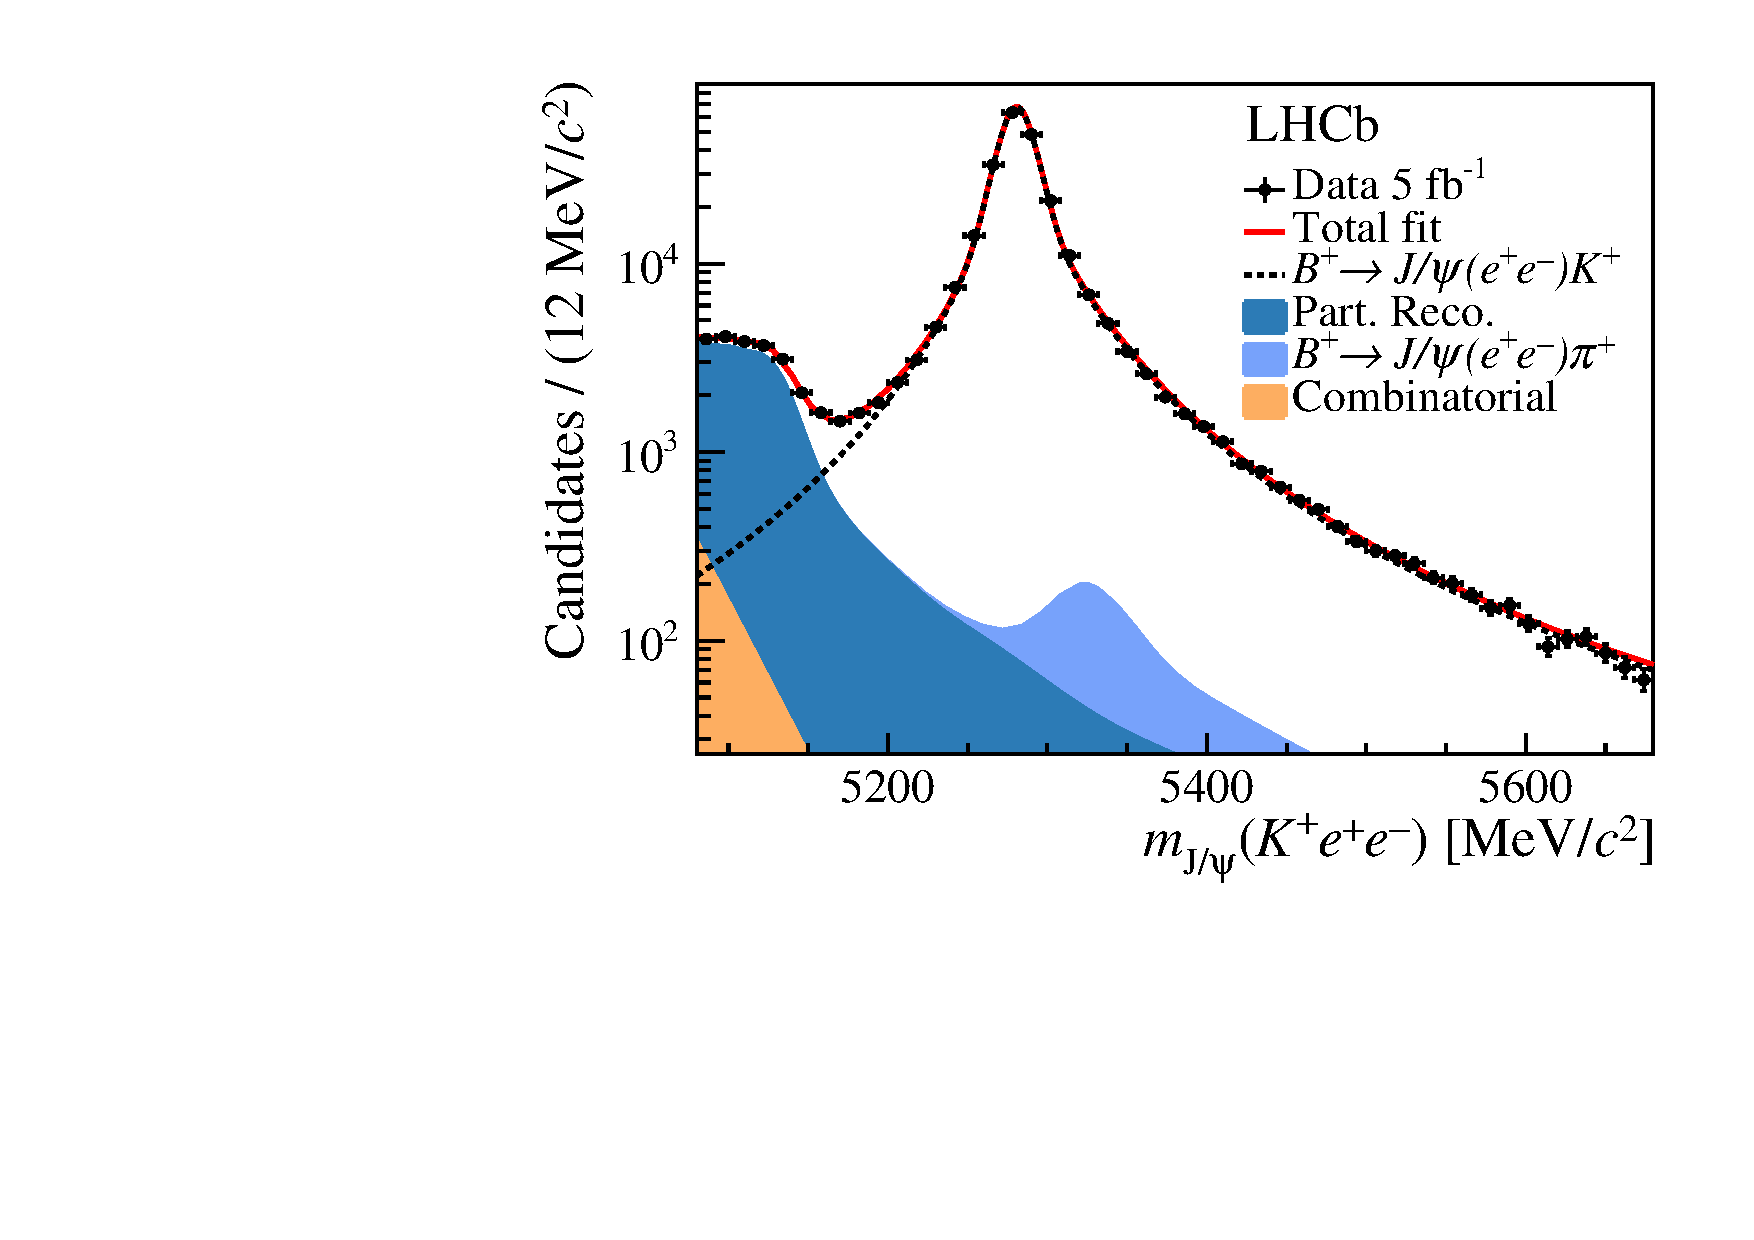
\includegraphics[width=0.45\textwidth]{figures/Fig7c.pdf}
    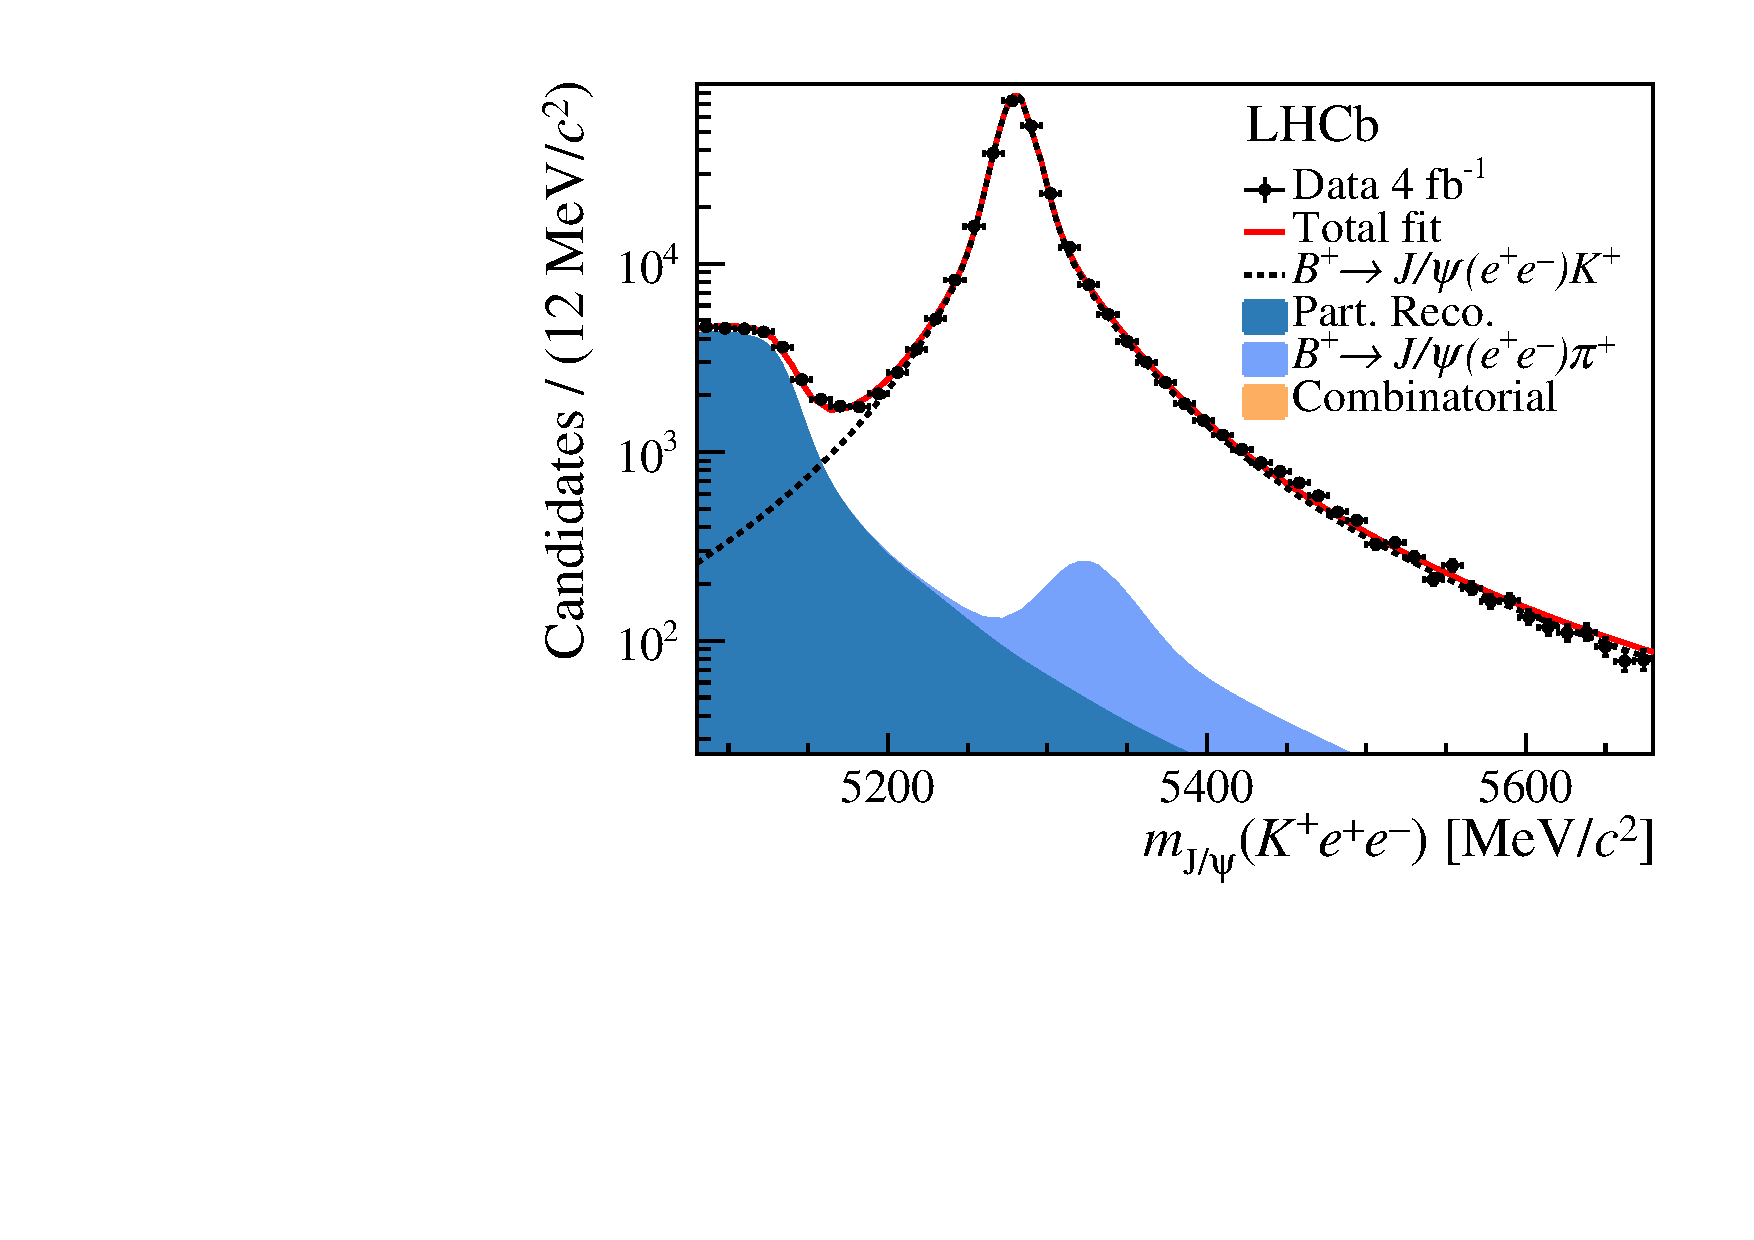
\includegraphics[width=0.45\textwidth]{figures/Fig7d.pdf}
    
    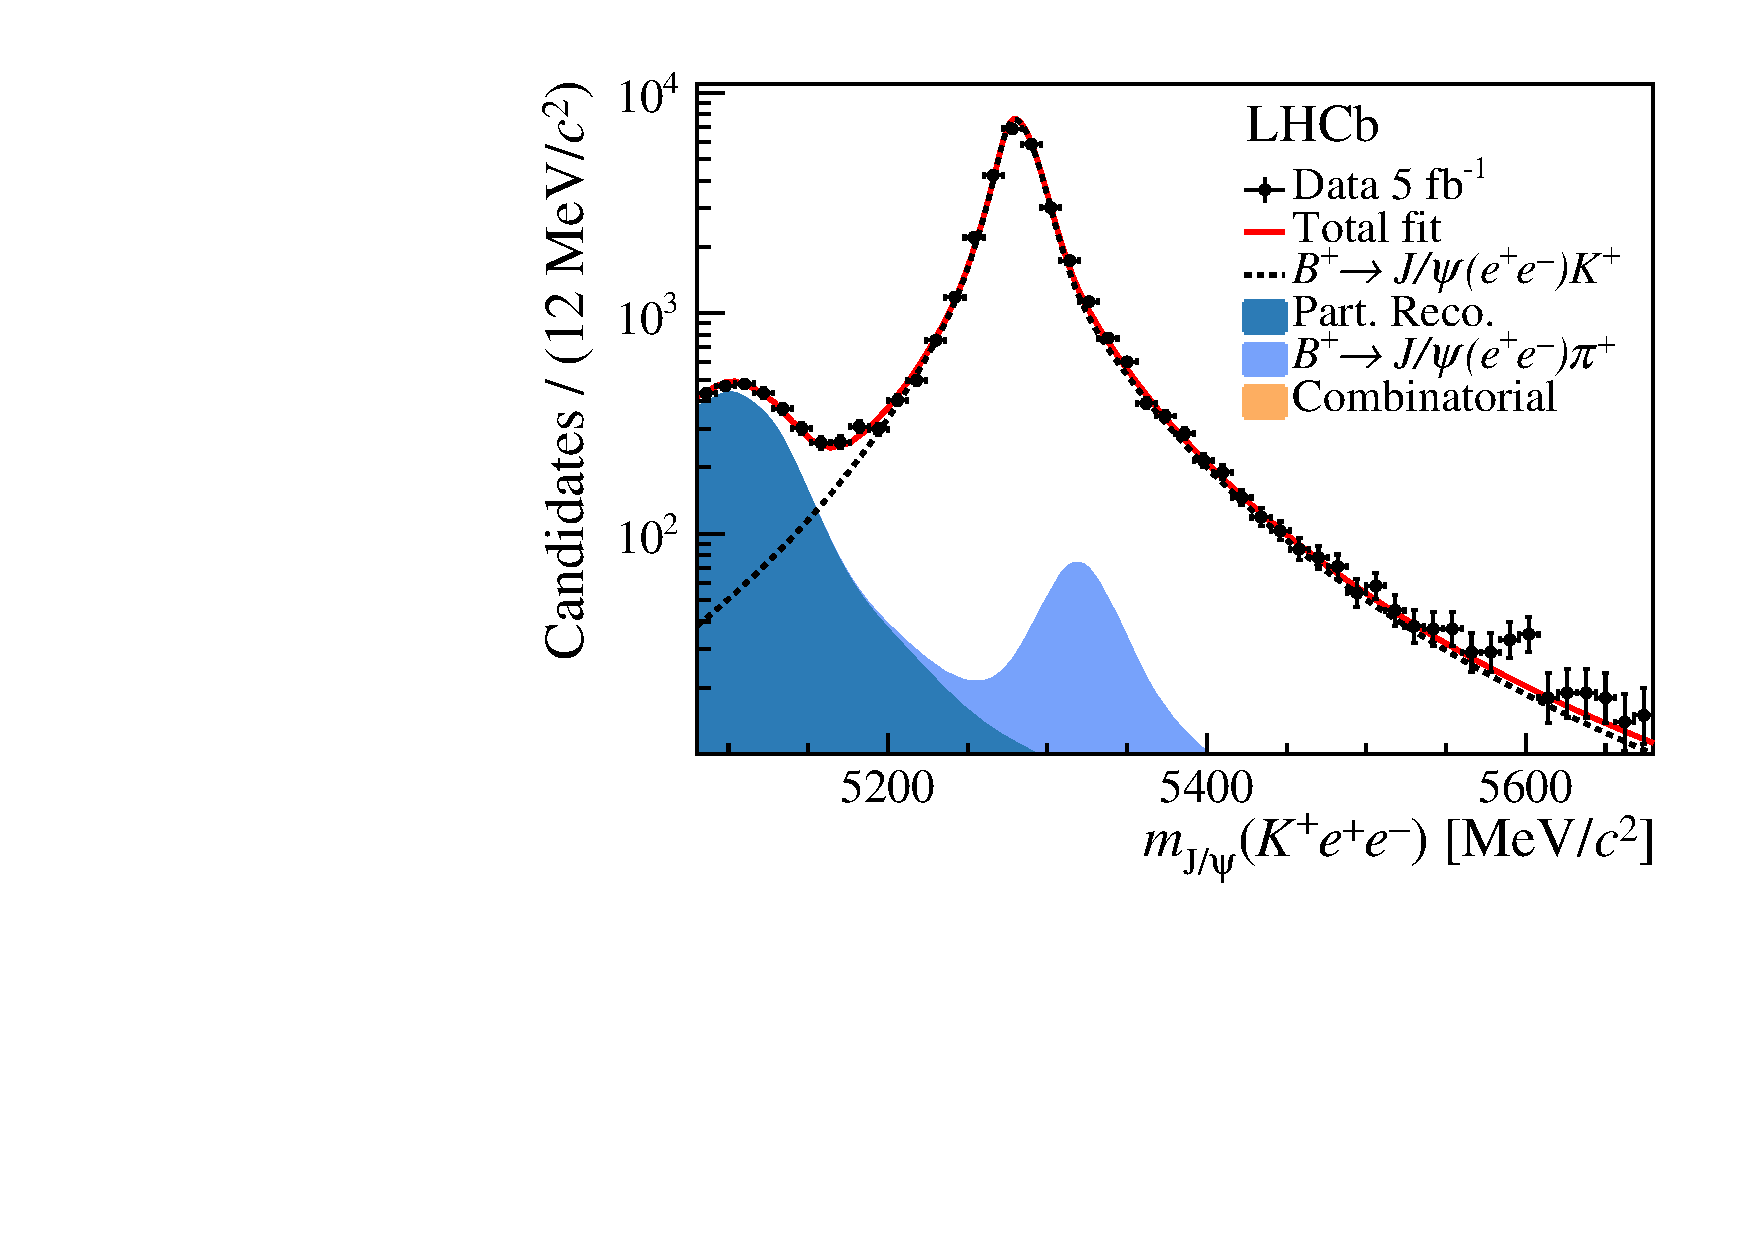
\includegraphics[width=0.45\textwidth]{figures/Fig7e.pdf}
    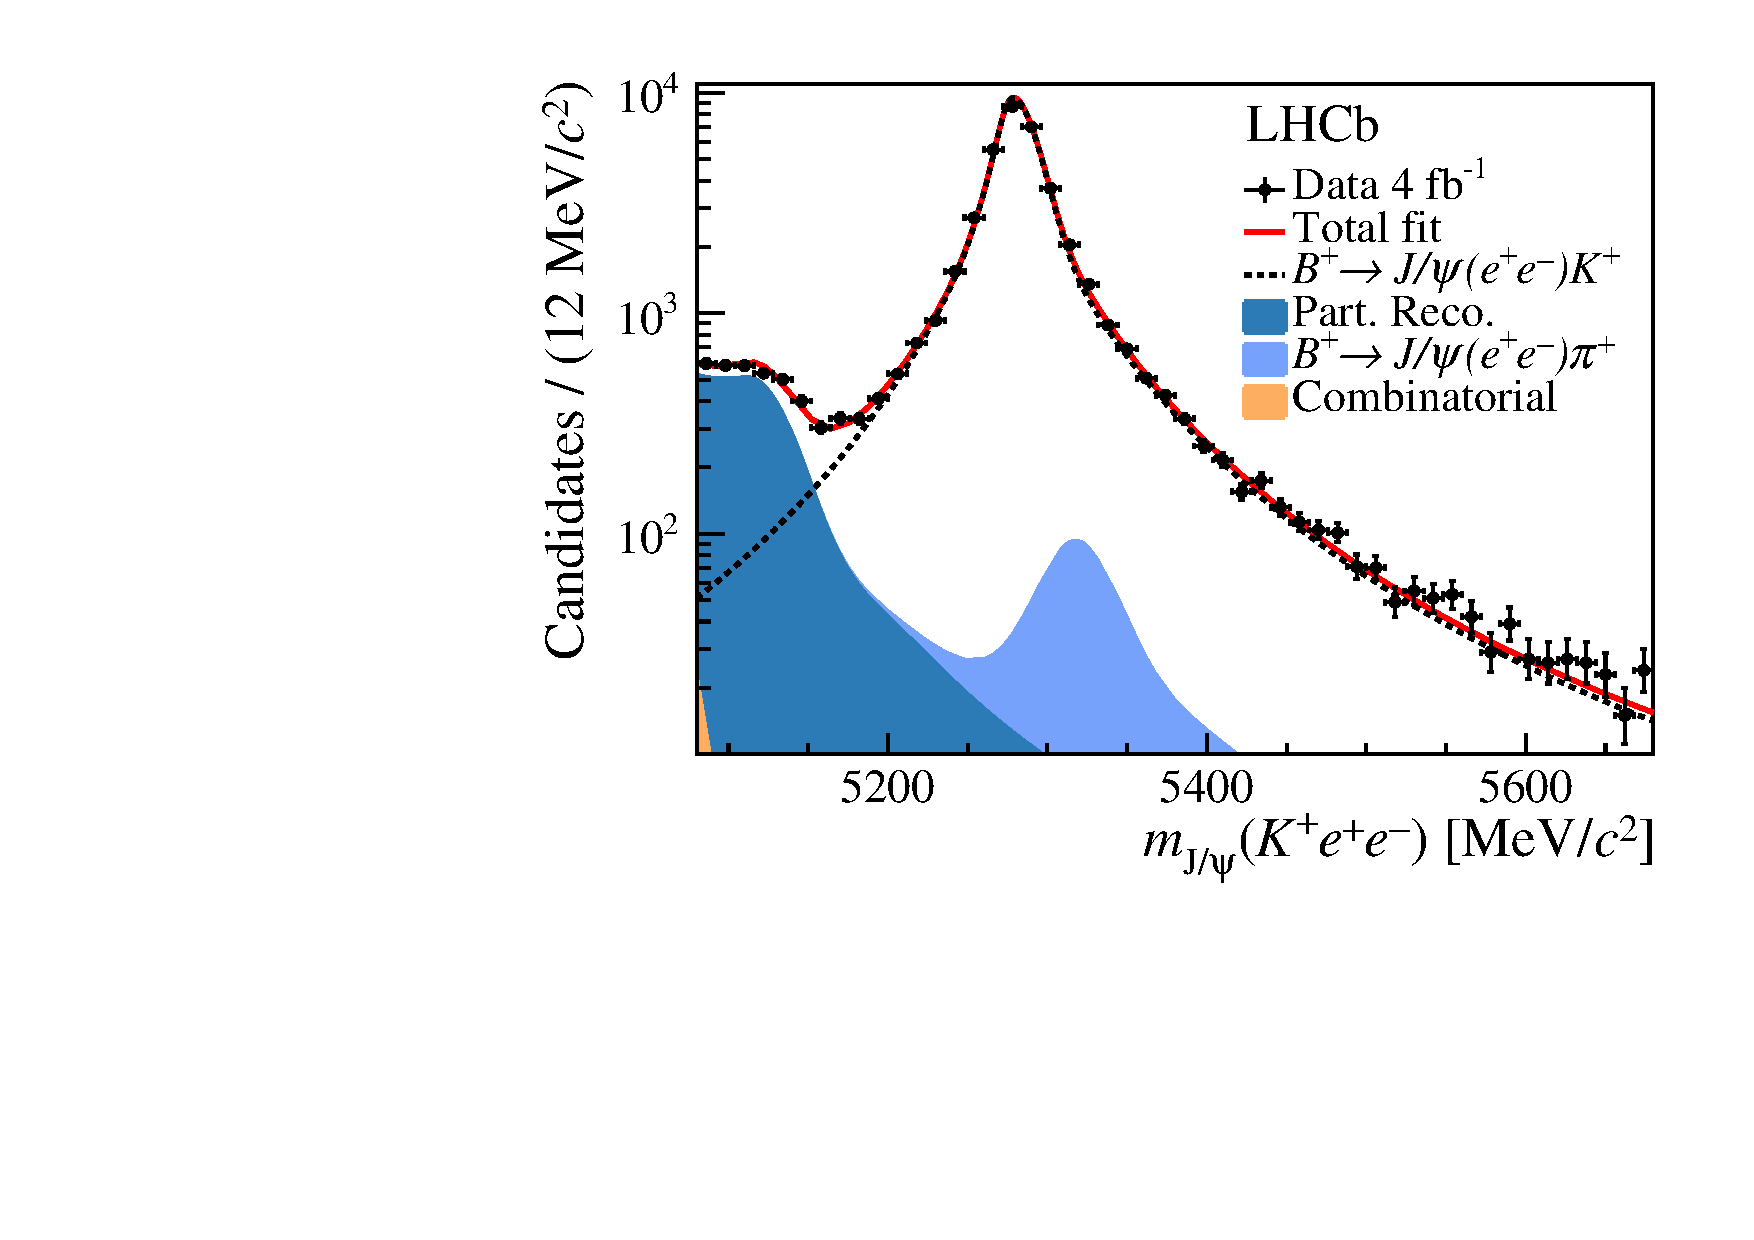
\includegraphics[width=0.45\textwidth]{figures/Fig7f.pdf}
    
    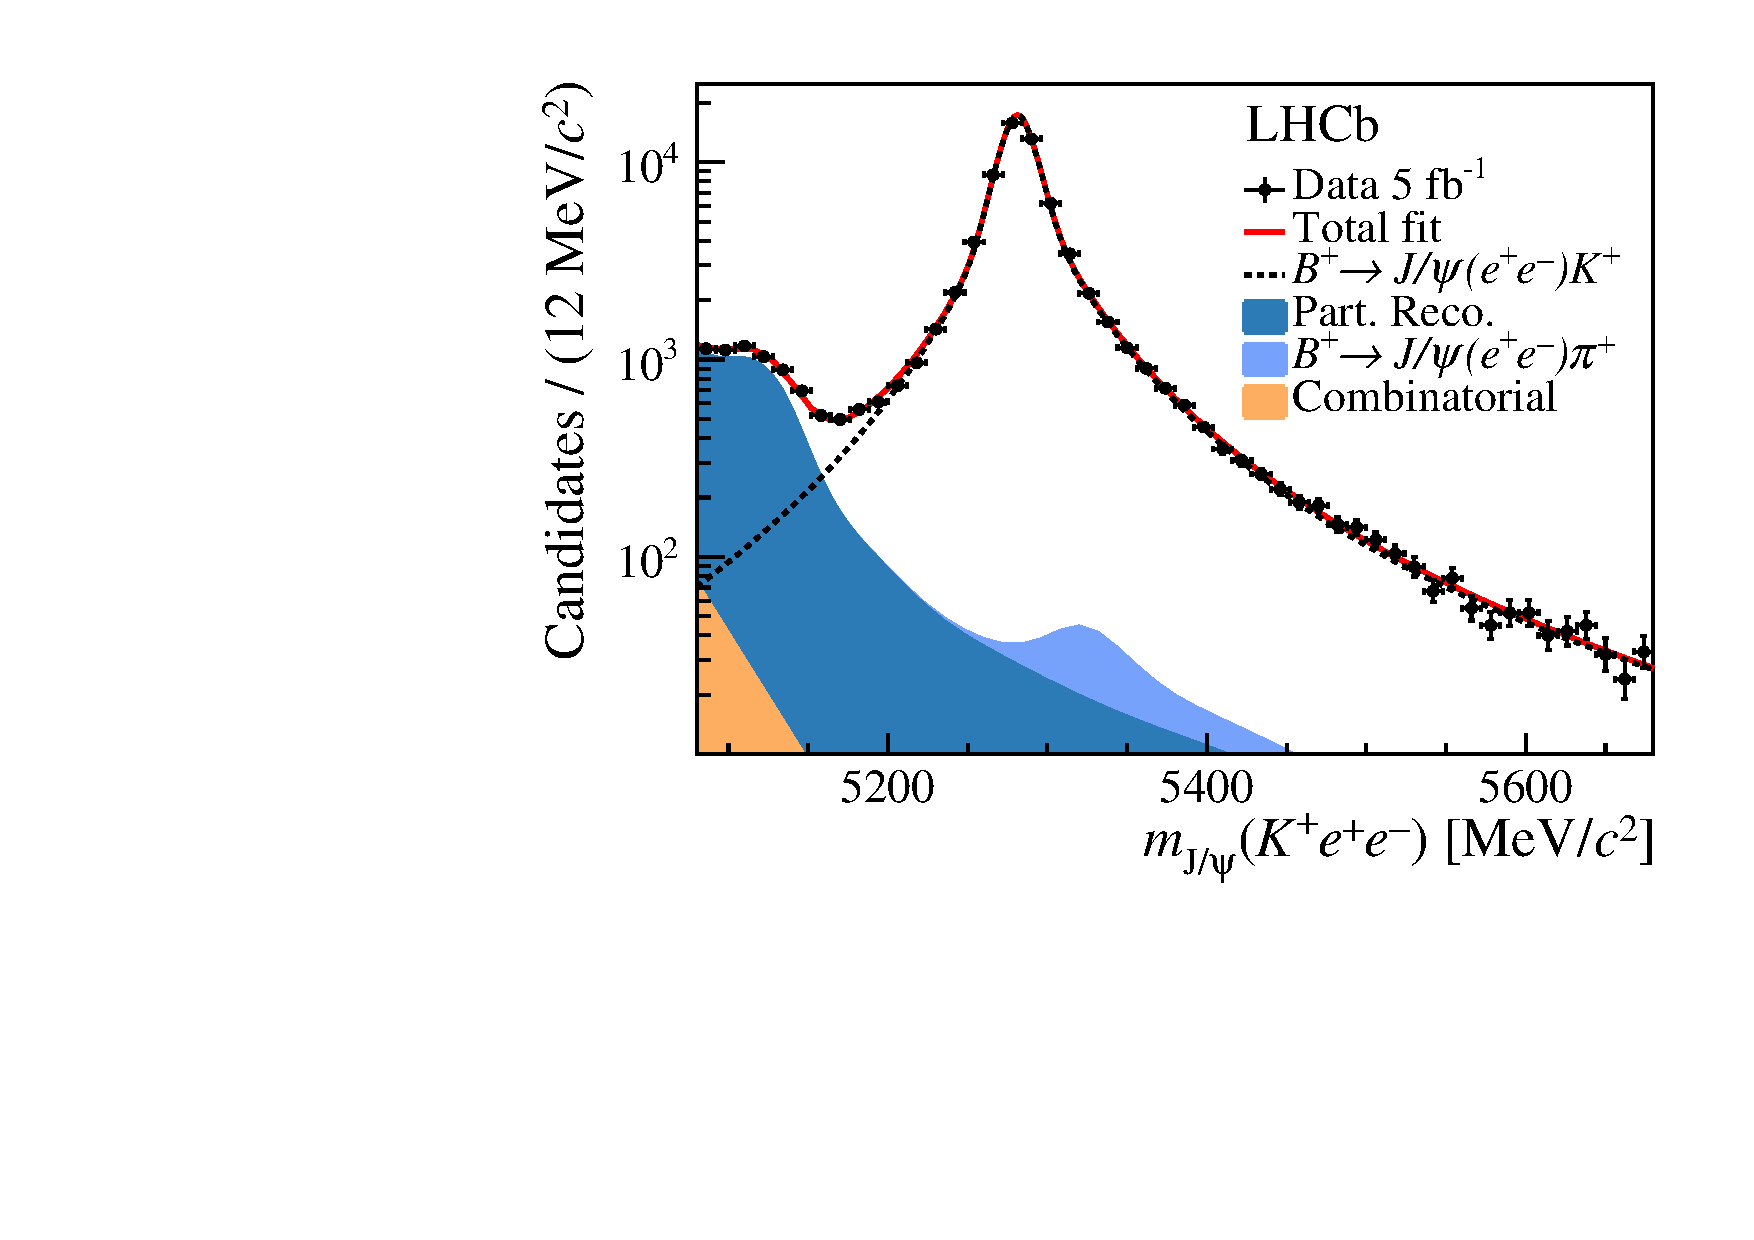
\includegraphics[width=0.45\textwidth]{figures/Fig7g.pdf}
    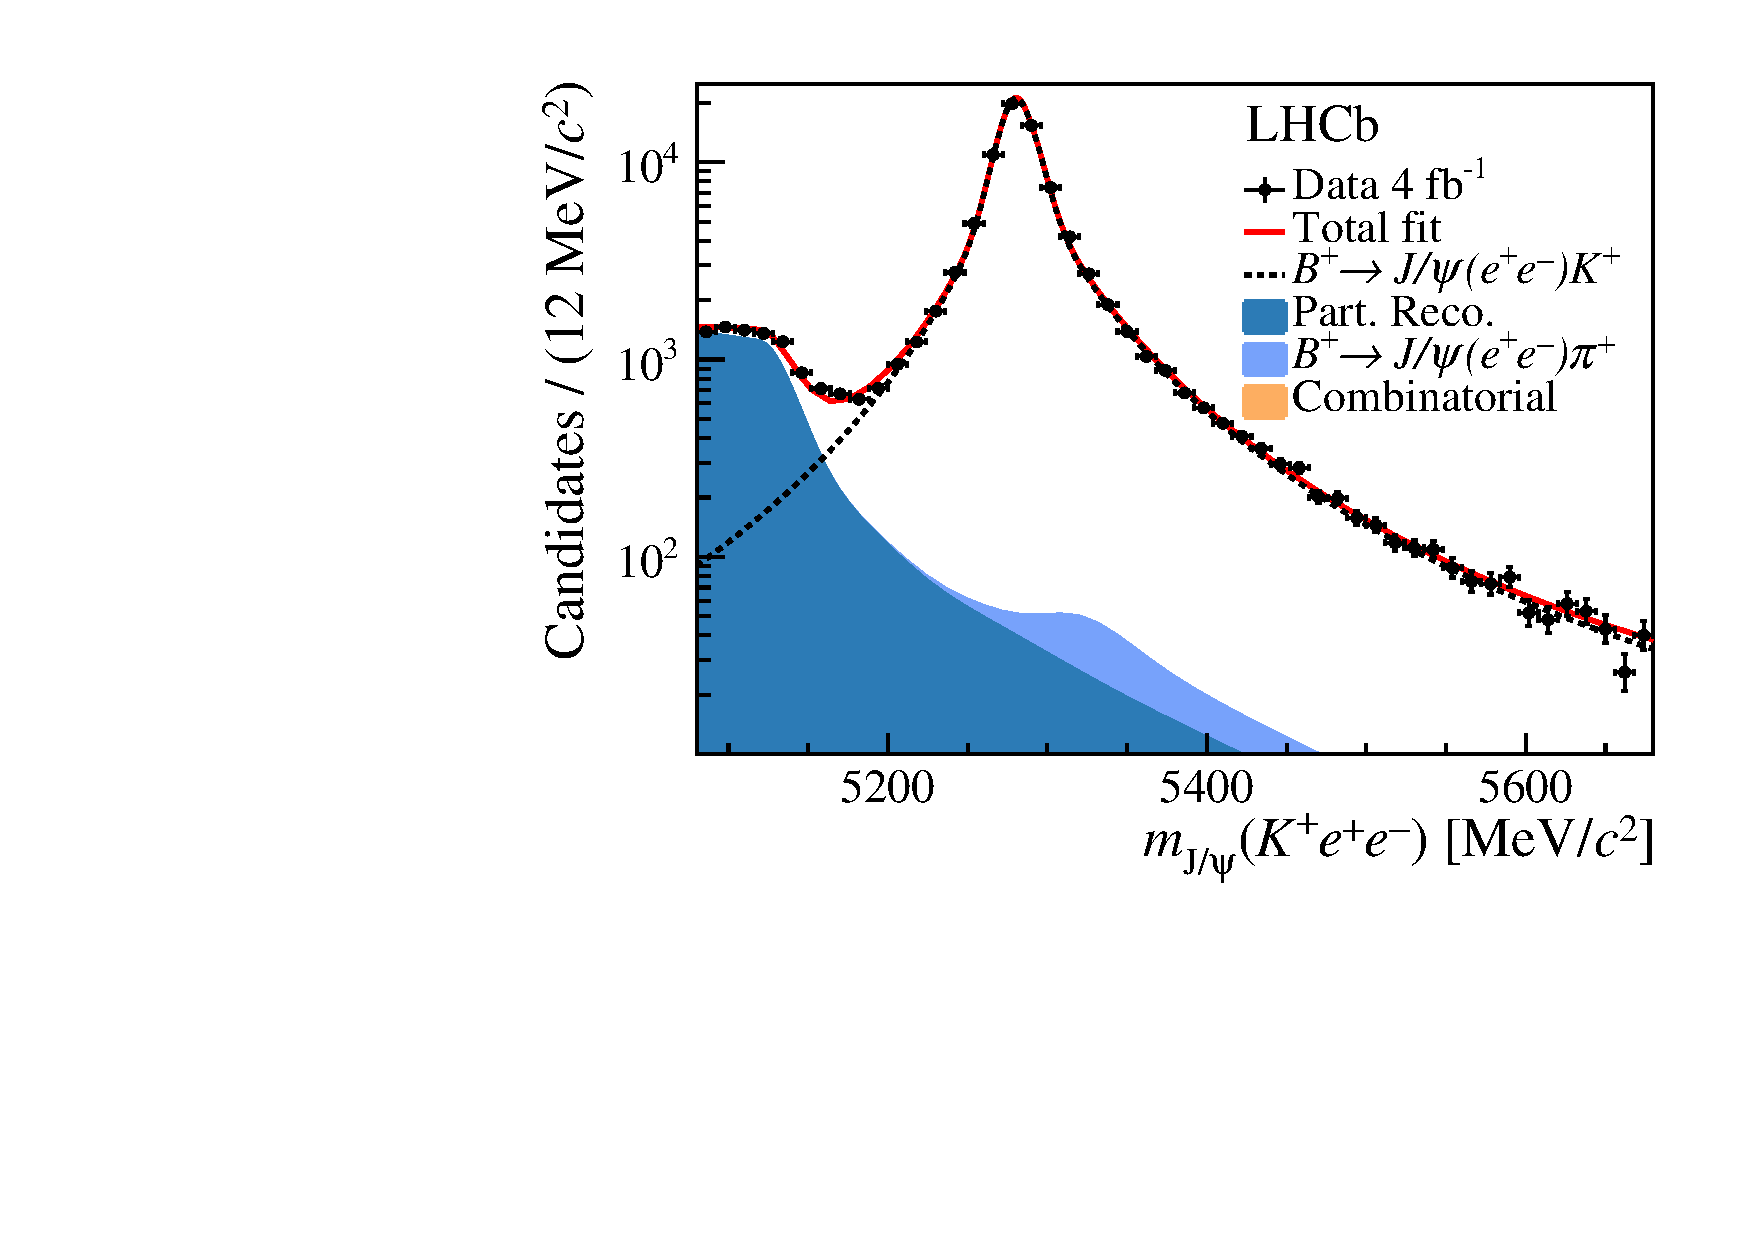
\includegraphics[width=0.45\textwidth]{figures/Fig7h.pdf}
    
    \caption{Candidate invariant mass distributions. Distribution of the invariant mass \mKllconst for resonant candidates in the (left) sample previously analysed~\cite{LHCb-PAPER-2019-009} and (right) the new data sample. The top row shows the fit to the muon modes and the subsequent rows the fits to the electron modes triggered by (second row) one of the electrons, (third row) the kaon and (last row) by other particles in the event. The fit projections are superimposed.
}
    \label{fig:resfits_categories}
\end{figure}


The profile likelihood for the fit to the nonresonant decays is shown in Fig.~\ref{fig:profile_likelihood}. The likelihood is non-Gaussian in the region $\RK>0.95$ due to the comparatively low yield of \BuKee events. 
Following the procedure described in Refs.~\cite{LHCb-PAPER-2019-009, LHCb-PAPER-2017-013}, the p-value is computed by integrating the posterior probability density function for \RK, having folded in the theory uncertainty on the SM prediction, for \RK values larger than the SM  expectation. The corresponding significance in terms of standard deviations is computed using the inverse Gaussian cumulative distribution function for a one-sided conversion.

A test statistic is constructed that is based on the likelihood ratio between two hypotheses with common (null) or different (test) \RK values for the part of the sample analysed previously (7, 8 and part of the 13\tev data) and for the new portion of the 13\tev data. Using pseudoexperiments based on the null hypothesis, the data suggest that the \RK value from the new portion of the data is compatible with that from the previous sample with a p-value of 95\%. Further tests give good compatibility for subsamples of the data corresponding to different trigger categories and magnet polarities.

The departure of the profile likelihood shown in Fig.~\ref{fig:profile_likelihood} from a normal distribution stems from the  definition of \RK. In particular,
in the \RK ratio the denominator is affected by larger statistical uncertainties than the numerator, owing to the larger number of nonresonant muonic signal candidates. However, the intervals of the likelihood distribution are found to be the same when estimated with $1/\RK$ as the fit parameter.


\begin{figure}[!t]
   \begin{center}
      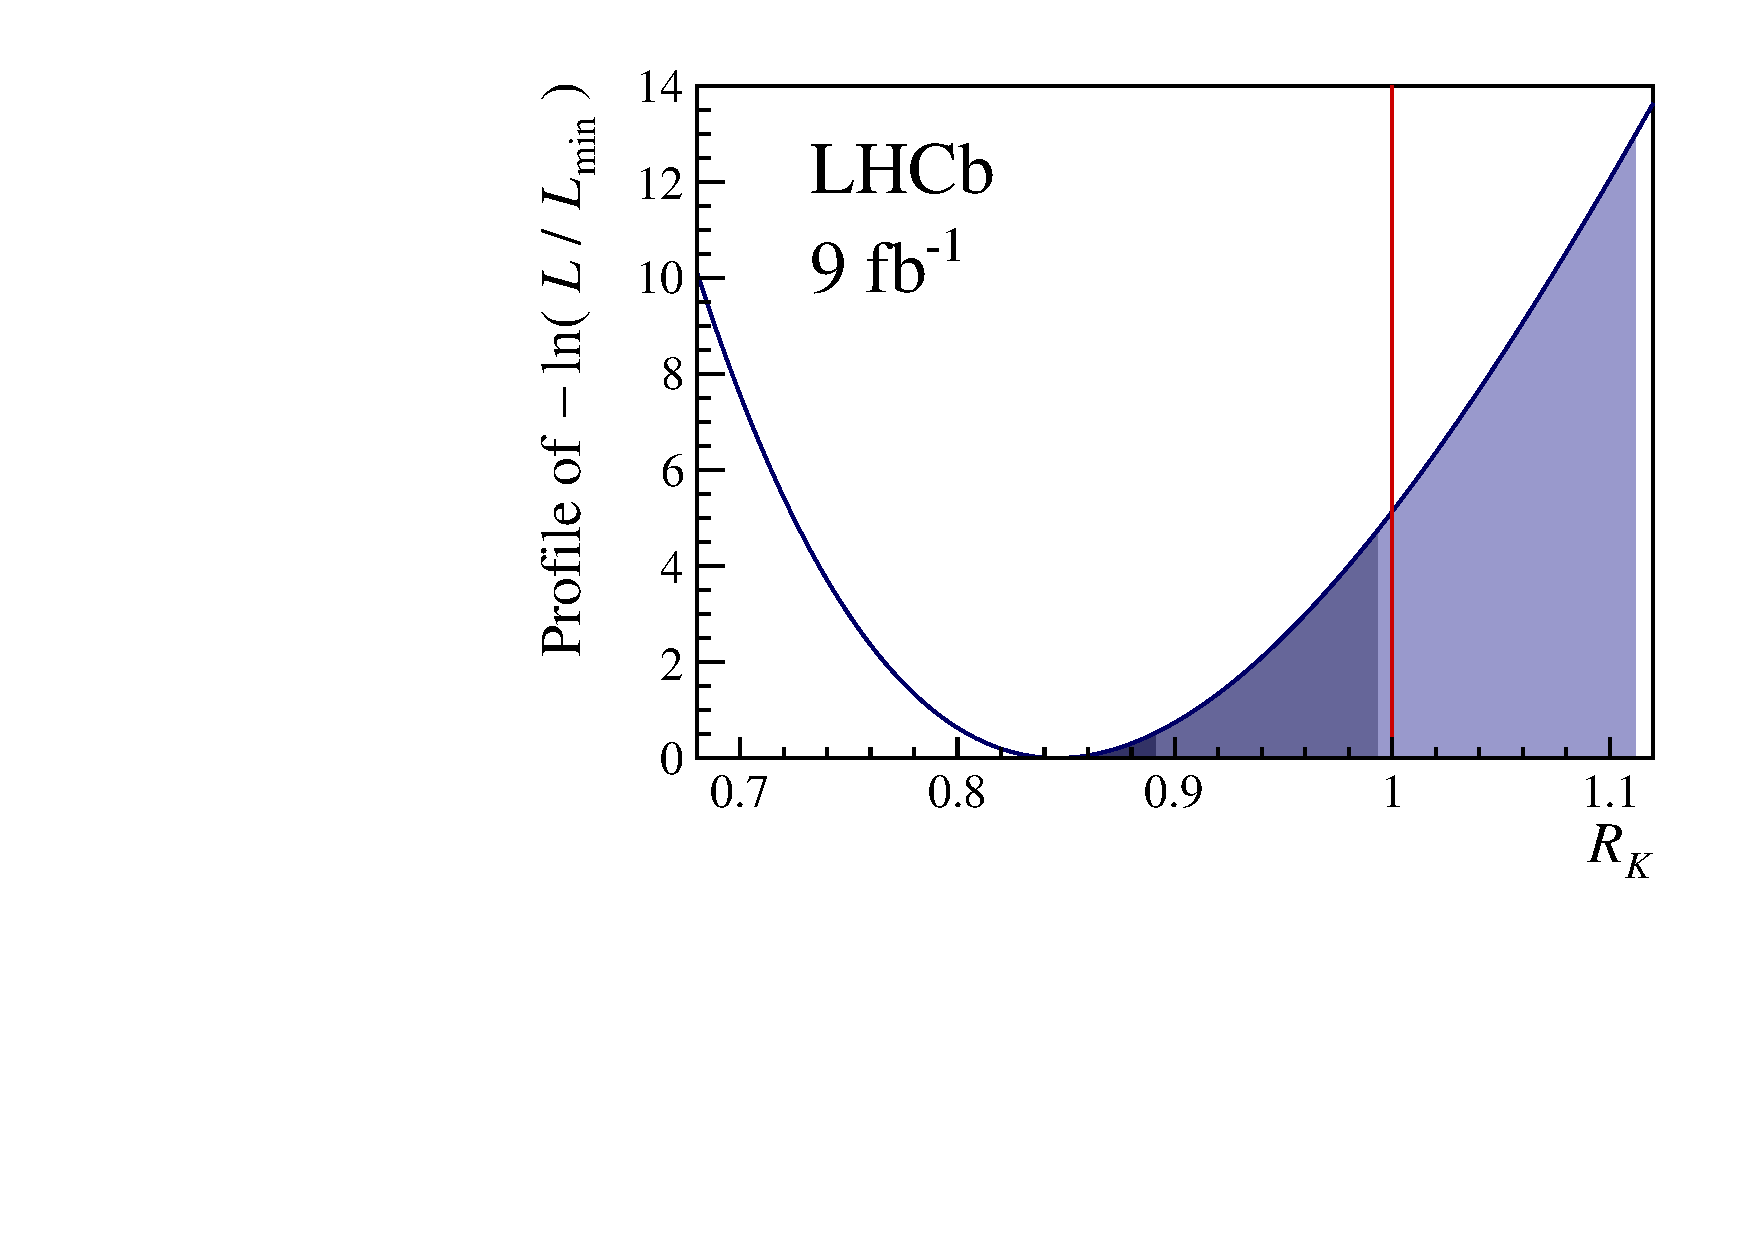
\includegraphics[height=0.25\textheight]{figures/Fig8.pdf}
  \end{center}
     \caption{Likelihood function from the fit to the nonresonant \BuKll candidates profiled as a function of \RK. The extent of the  dark, medium and light blue  regions shows the values allowed for \RK at $1\sigma$, $3\sigma$ and $5\sigma$ levels. The red line indicates the prediction from the SM. }
    \label{fig:profile_likelihood}
\end{figure}



\subsubsection*{Additional cross-checks} 

The \rjpsi single ratio is used to perform a number of additional cross-checks. The distribution of this ratio as a function of the angle between the leptons and the minimum \pt of the leptons is shown in Fig.~\ref{fig:rjpsi_differential1}, together with the spectra expected for the resonant and nonresonant decays.
No significant trend is observed in either \rjpsi distribution. Assuming the deviations observed are genuine mismodelling of the efficiencies, rather than statistical fluctuations, a total shift of \RK at a level less than $0.001$ would be expected due to these effects. This estimate takes into account the spectrum of the relevant variables in the nonresonant decay modes of interest and is compatible with the estimated systematic uncertainties on \RK. Similarly, the variations seen in \rjpsi as a function of all other reconstructed quantities examined are compatible with the systematic uncertainties assigned. In addition, \rjpsi is computed in two-dimensional intervals of reconstructed quantities, as shown in Fig.~\ref{fig:rjpsi_bin}. Again, no significant trend is seen.
 
\begin{figure}[!t]
   \begin{center}
   \begin{overpic}[width=0.45\linewidth,trim={0 0 0 0.5cm}, clip]{figures/Fig9a.pdf}
   \put(50,26){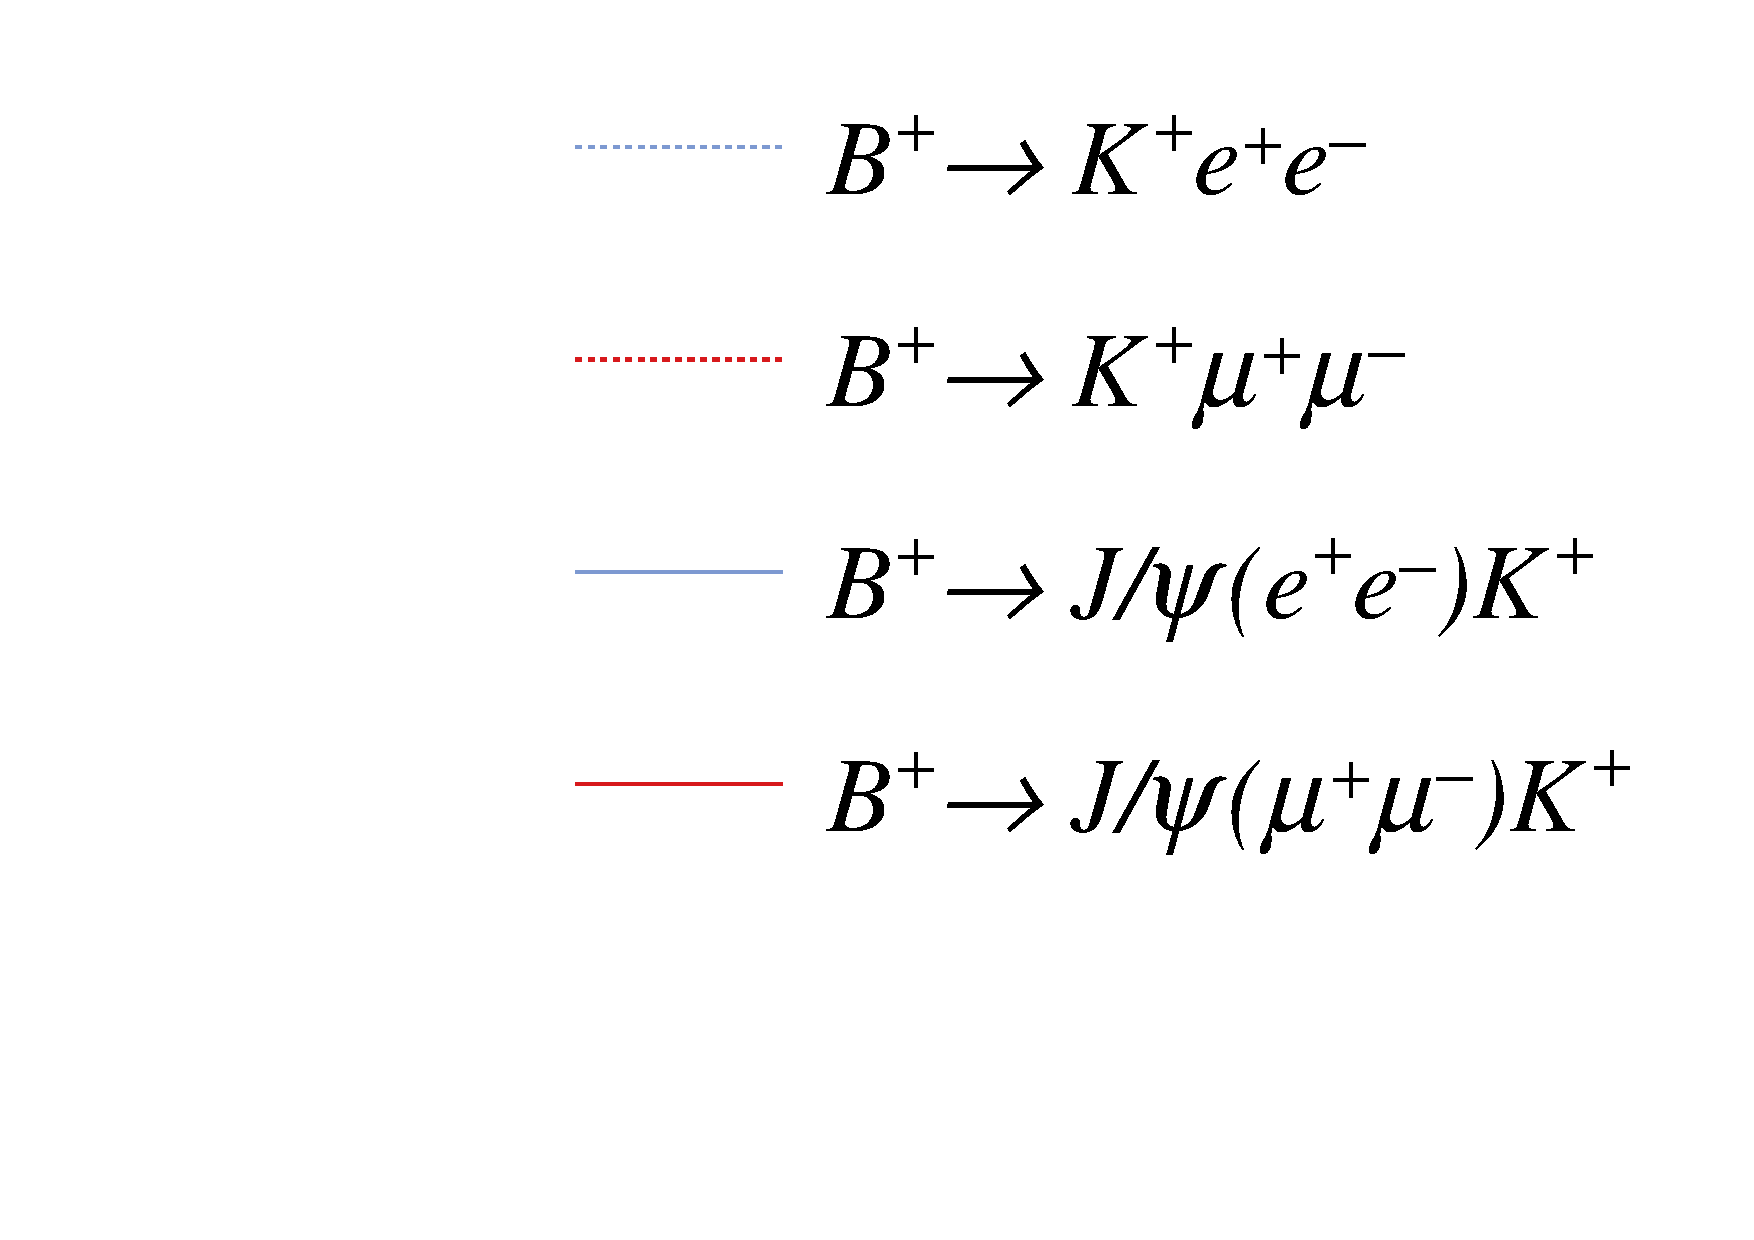
\includegraphics[width=0.2\linewidth]{figures/Fig9e.pdf}}
   \end{overpic}
   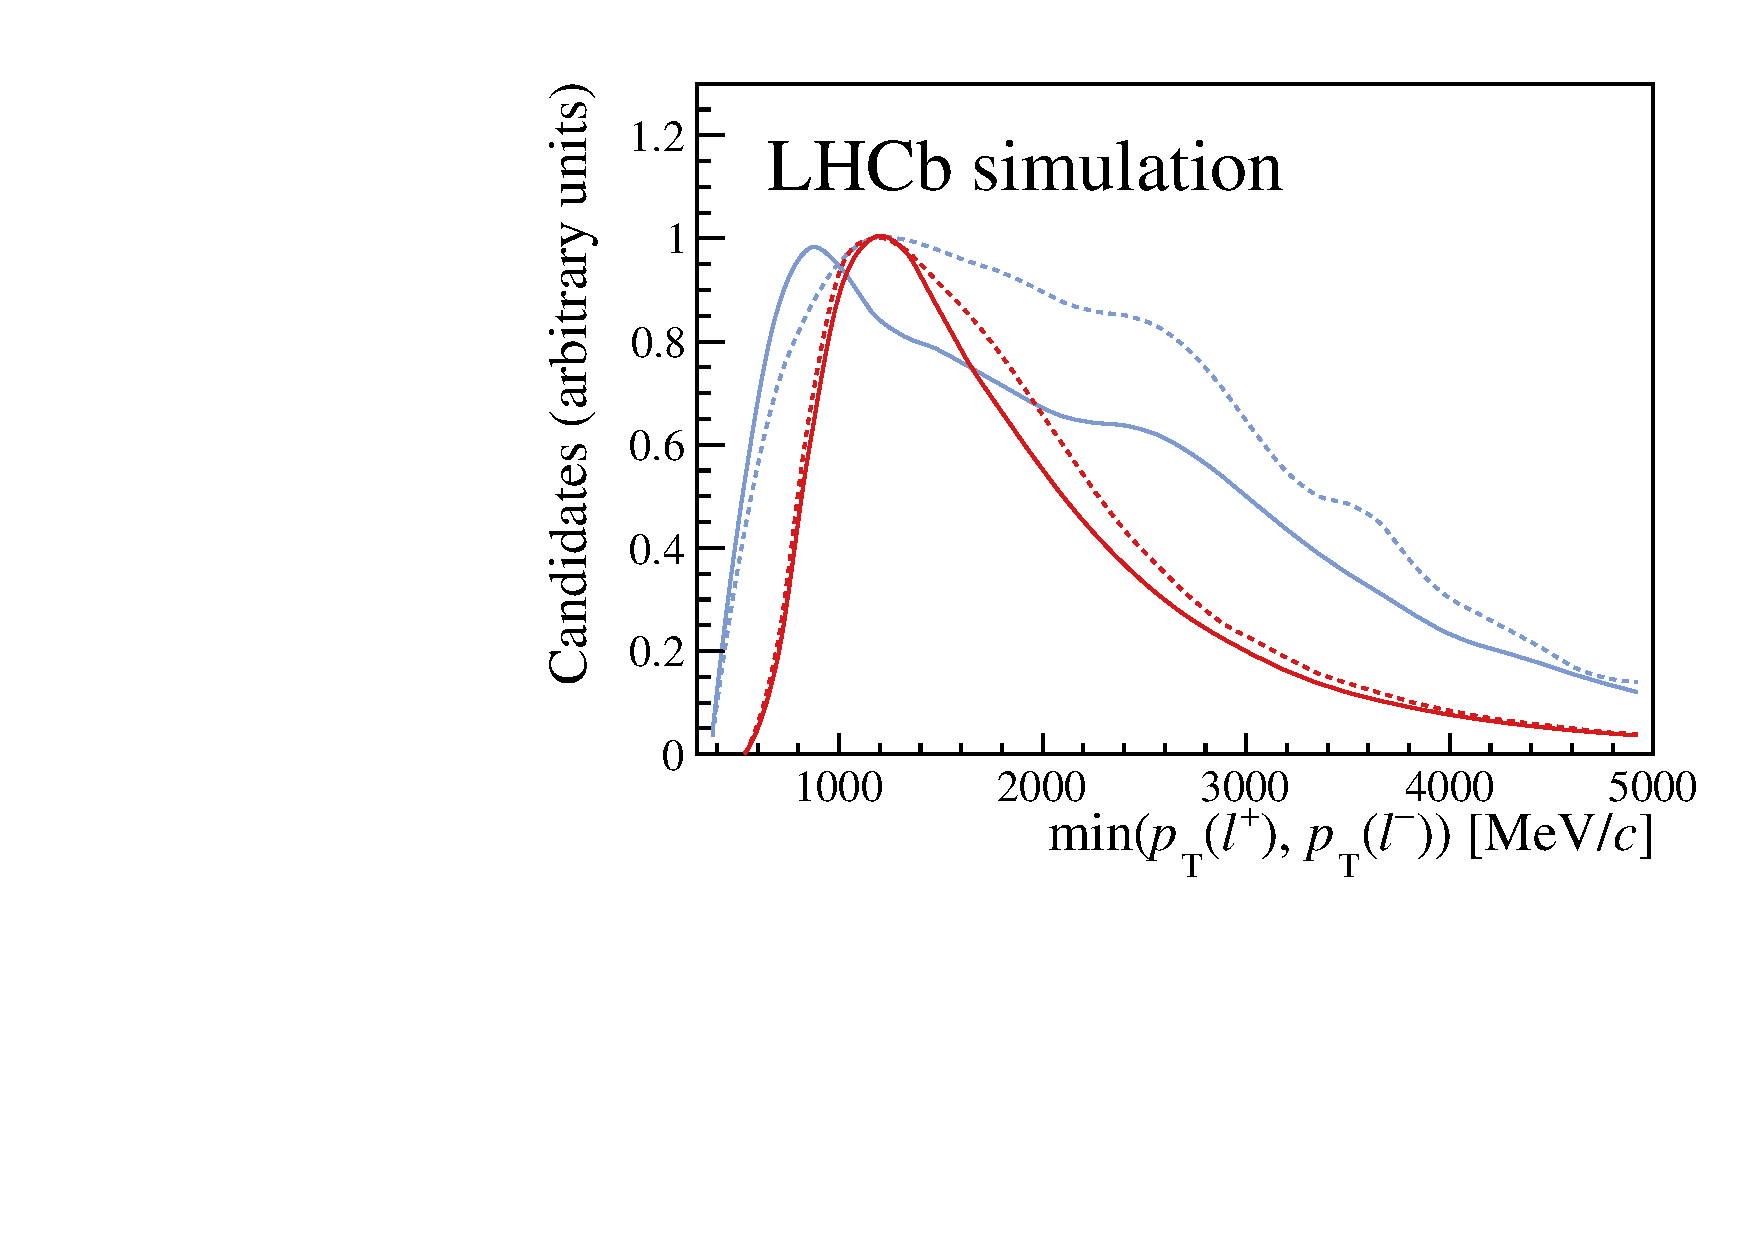
\includegraphics[width=0.45\linewidth,trim={0 0.15cm 0 0}, clip]{figures/Fig9b.pdf}
   
  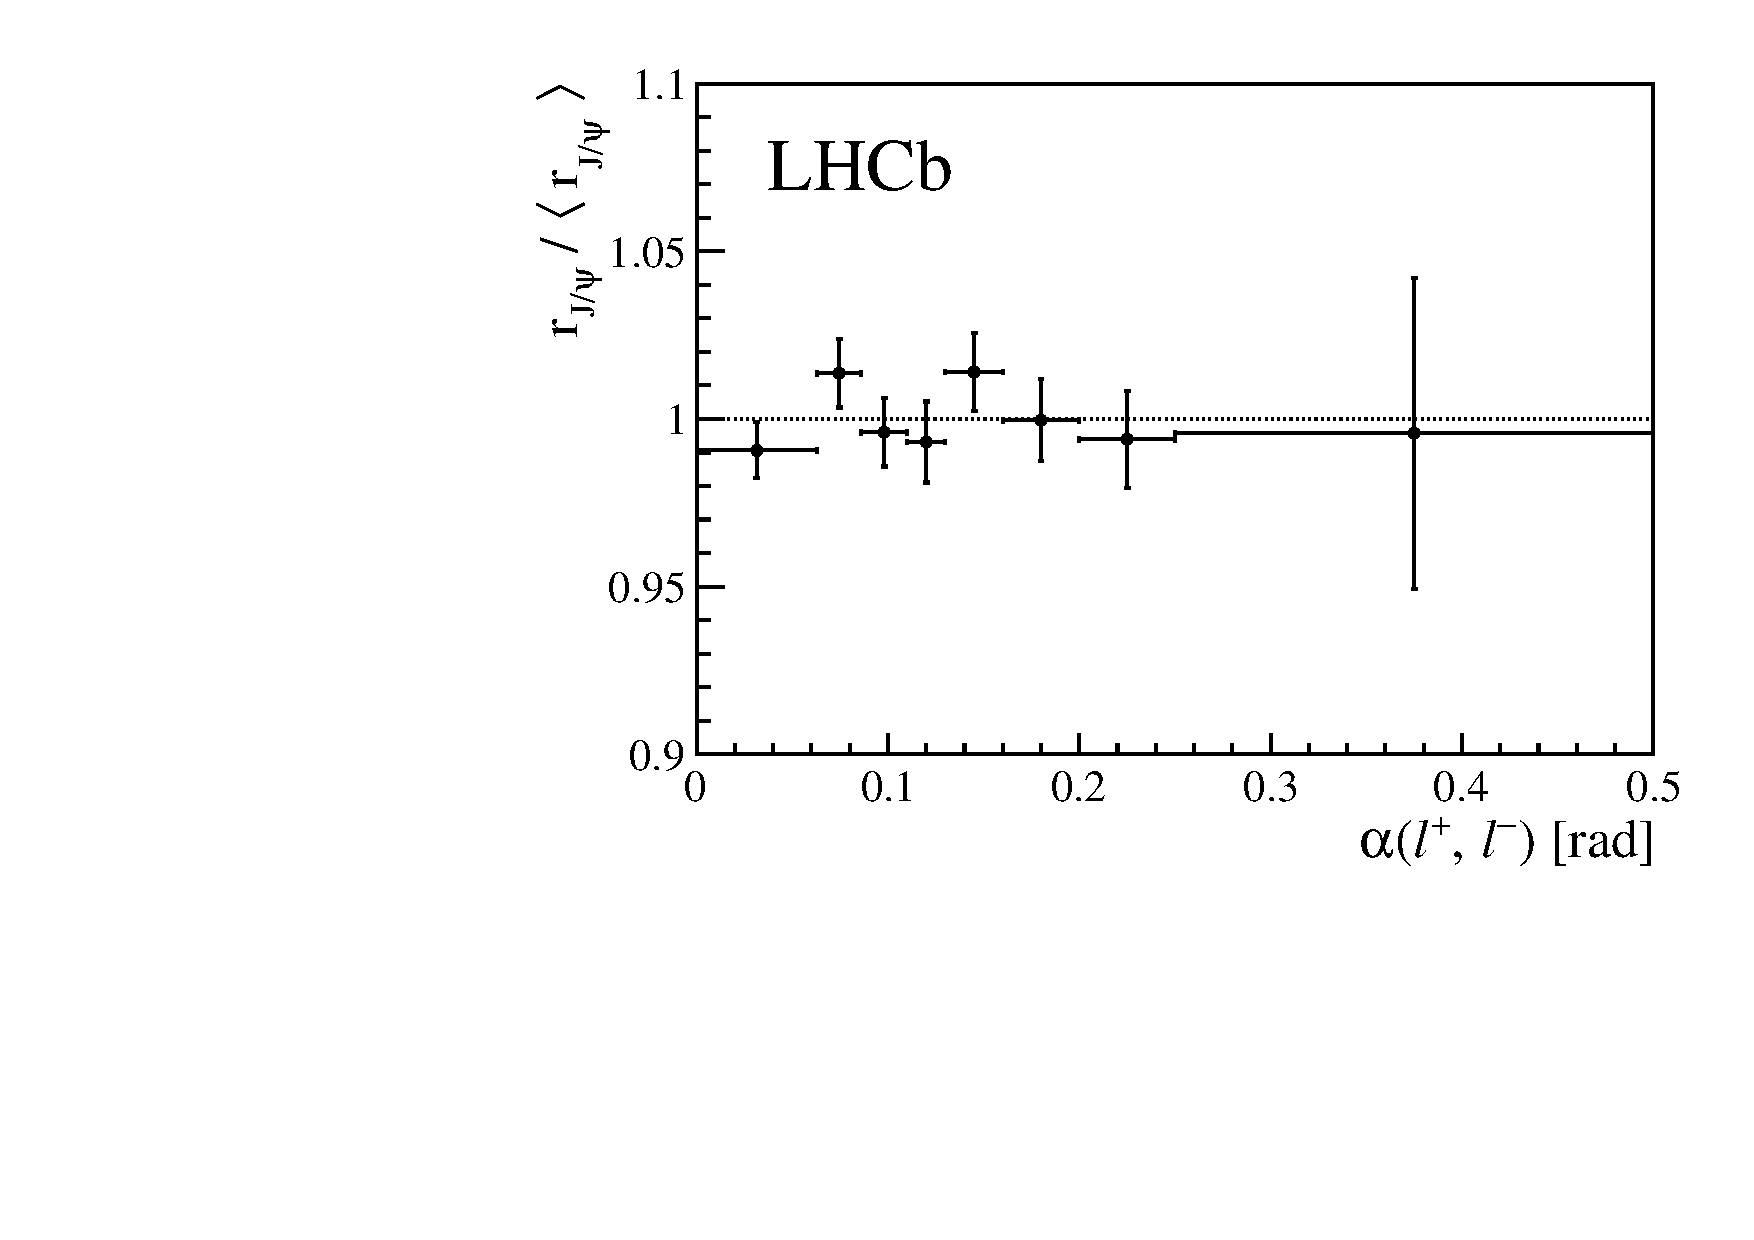
\includegraphics[width=0.45\linewidth,trim={0 0 0 0.5cm}, clip]{figures/Fig9c.pdf}
   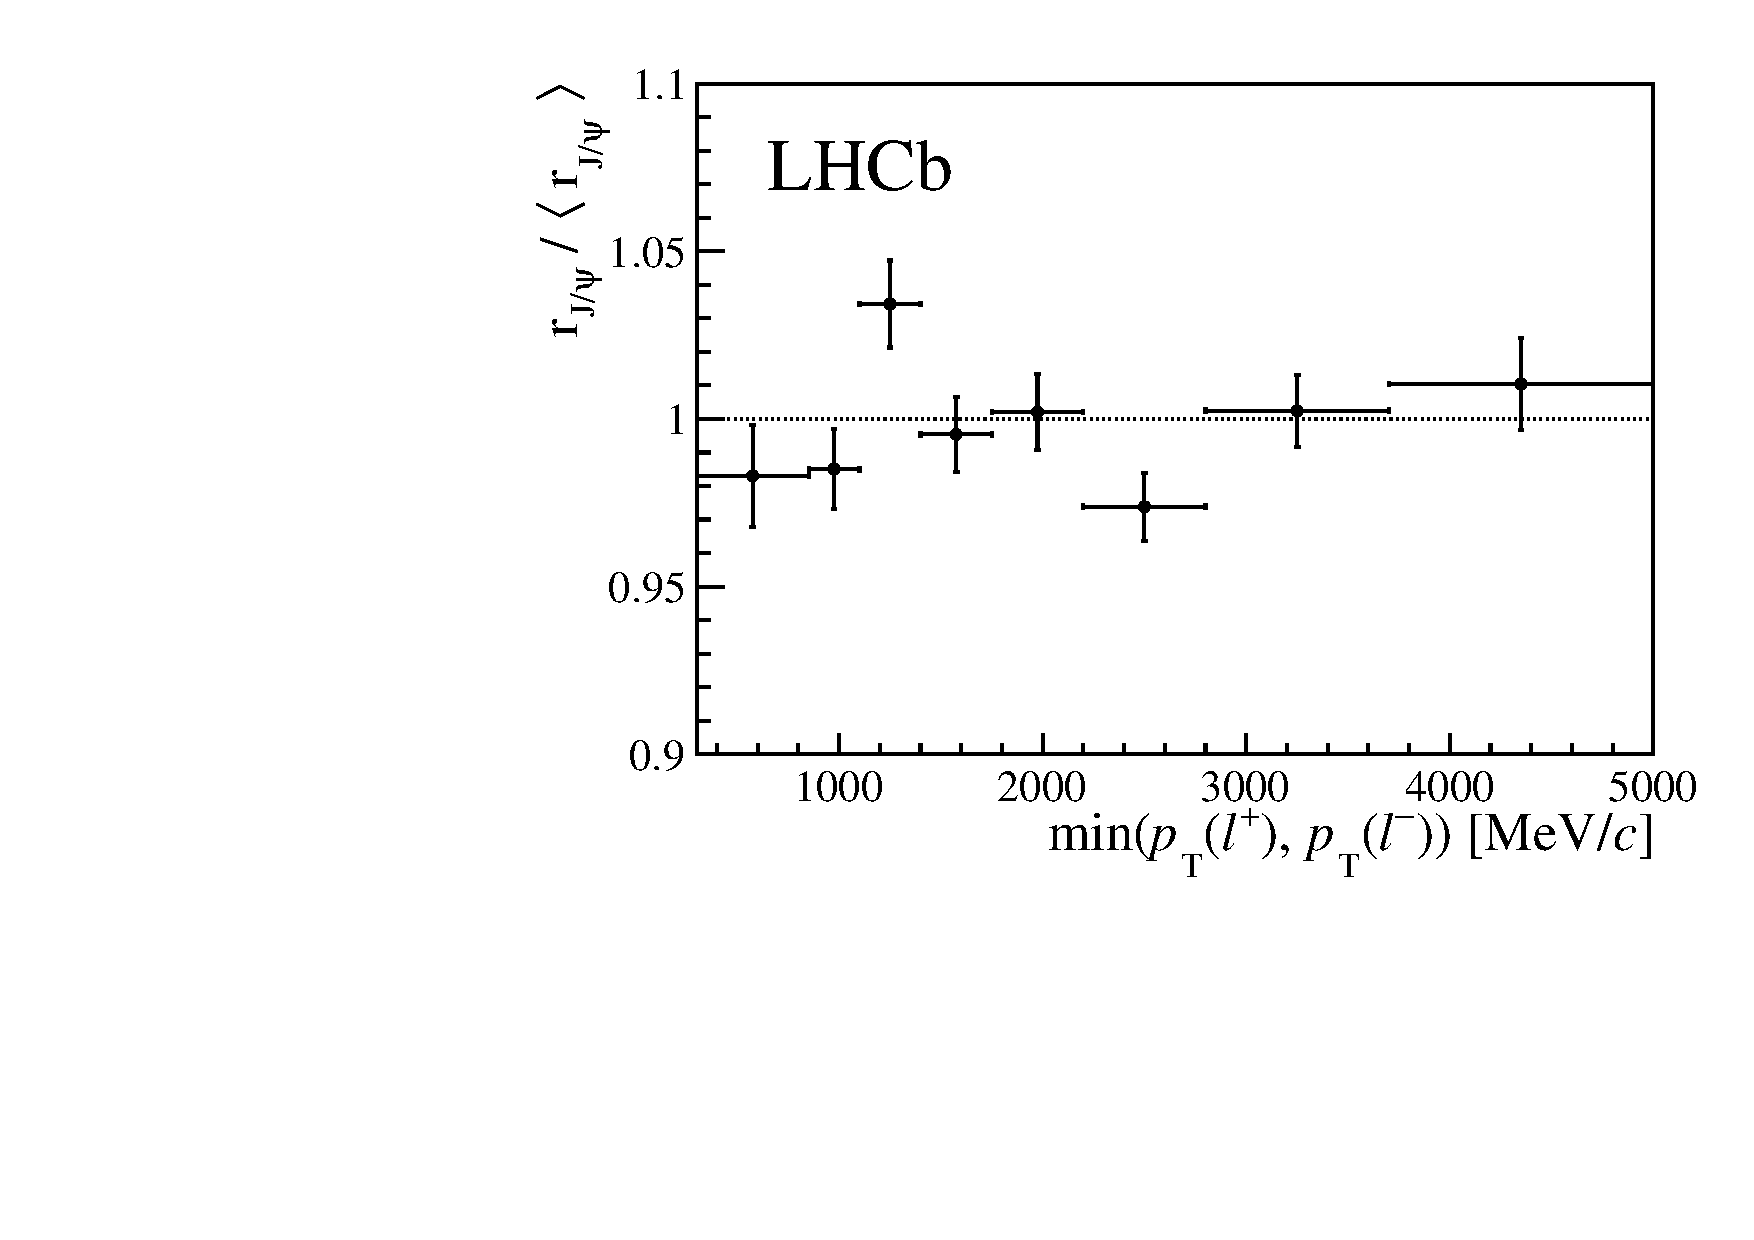
\includegraphics[width=0.45\linewidth,trim={0 0 0 0.5cm}, clip]{figures/Fig9d.pdf}
      \end{center}
     \caption{Differential \rjpsi measurement. (Top) distributions of the reconstructed spectra of (left) the angle between the leptons, and (right) the minimum \pt of the leptons. (Bottom) the single ratio \rjpsi relative to its average value $\left< \rjpsi \right>$ as a function of these variables. In the electron minimum \pt spectra, the structure at 2800\mevc is related to the trigger threshold.}
    \label{fig:rjpsi_differential1}
\end{figure}


\begin{figure}[!htbp]
   \begin{center}
   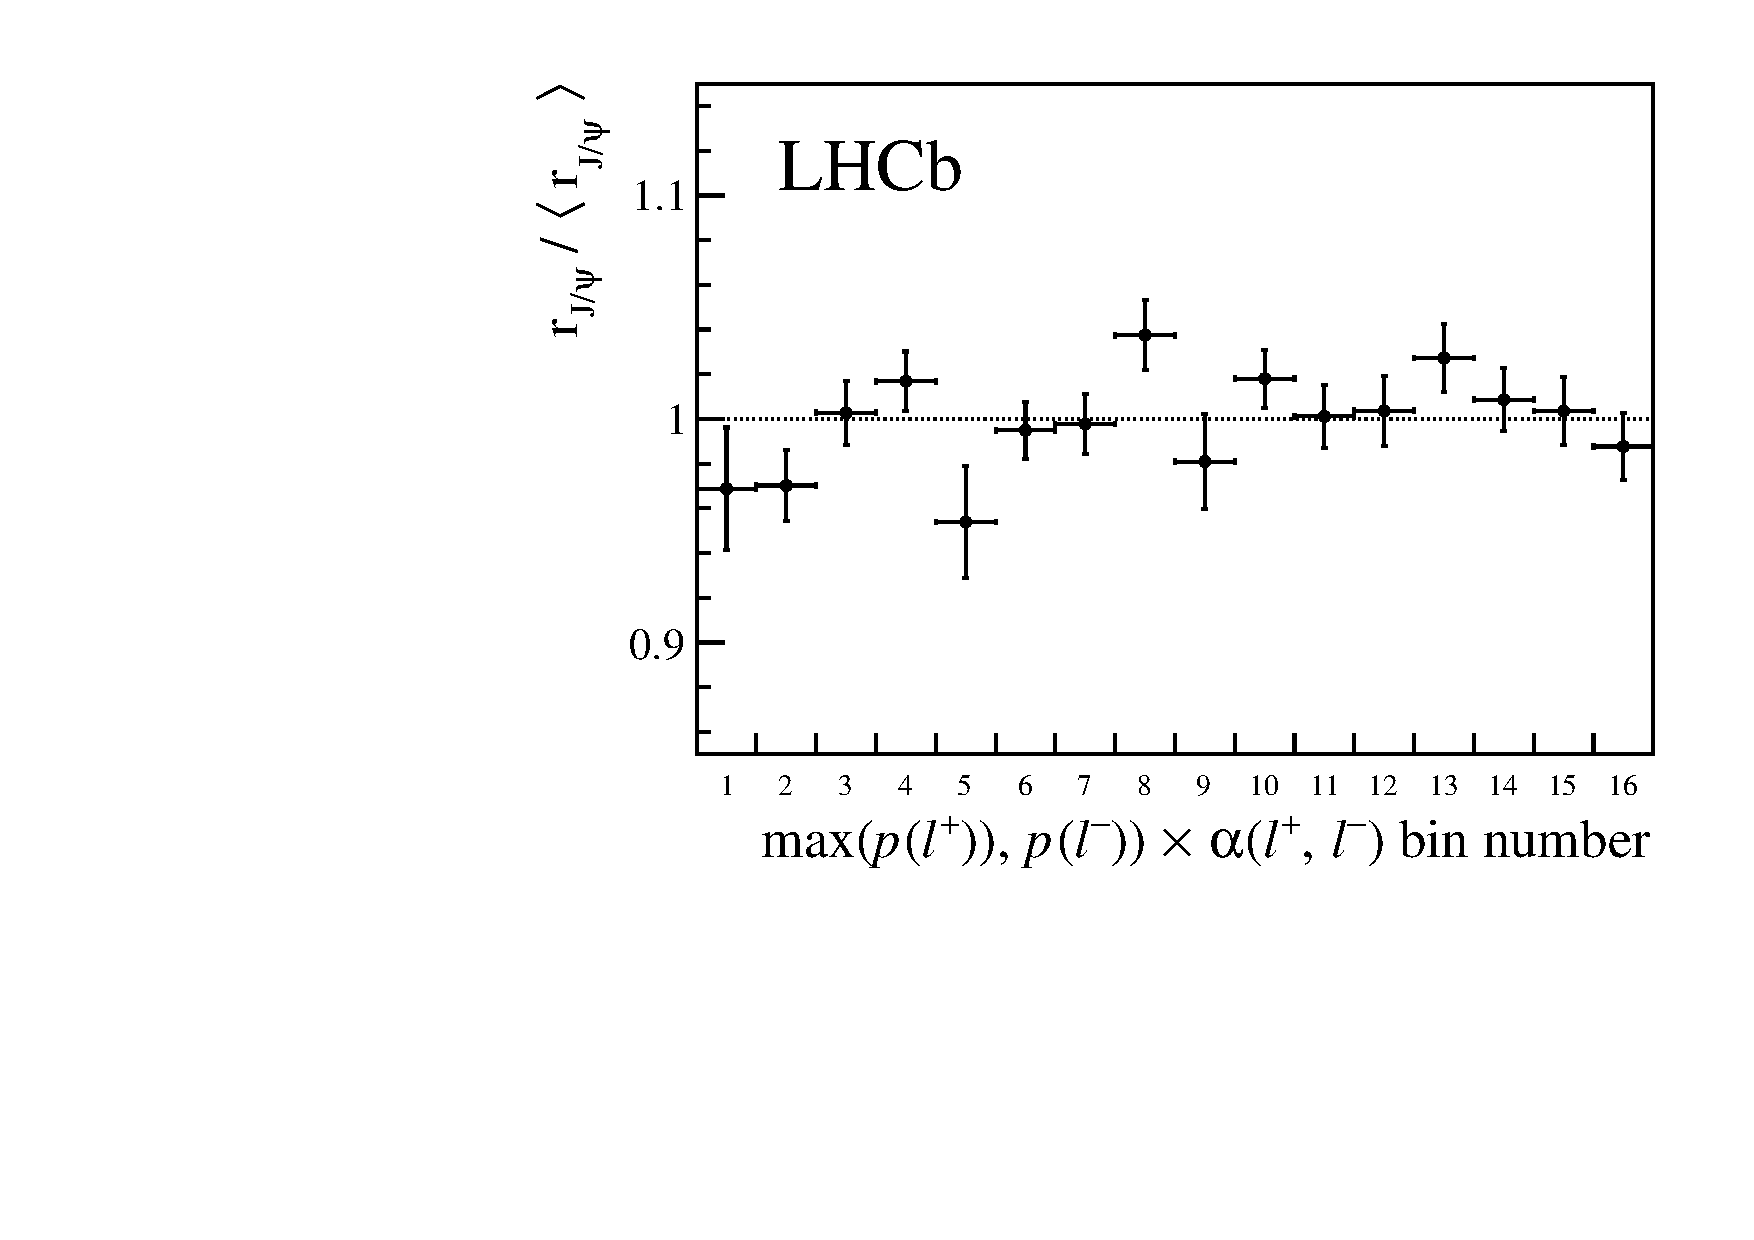
\includegraphics[width=0.45\linewidth]{figures/Fig10a.pdf}
    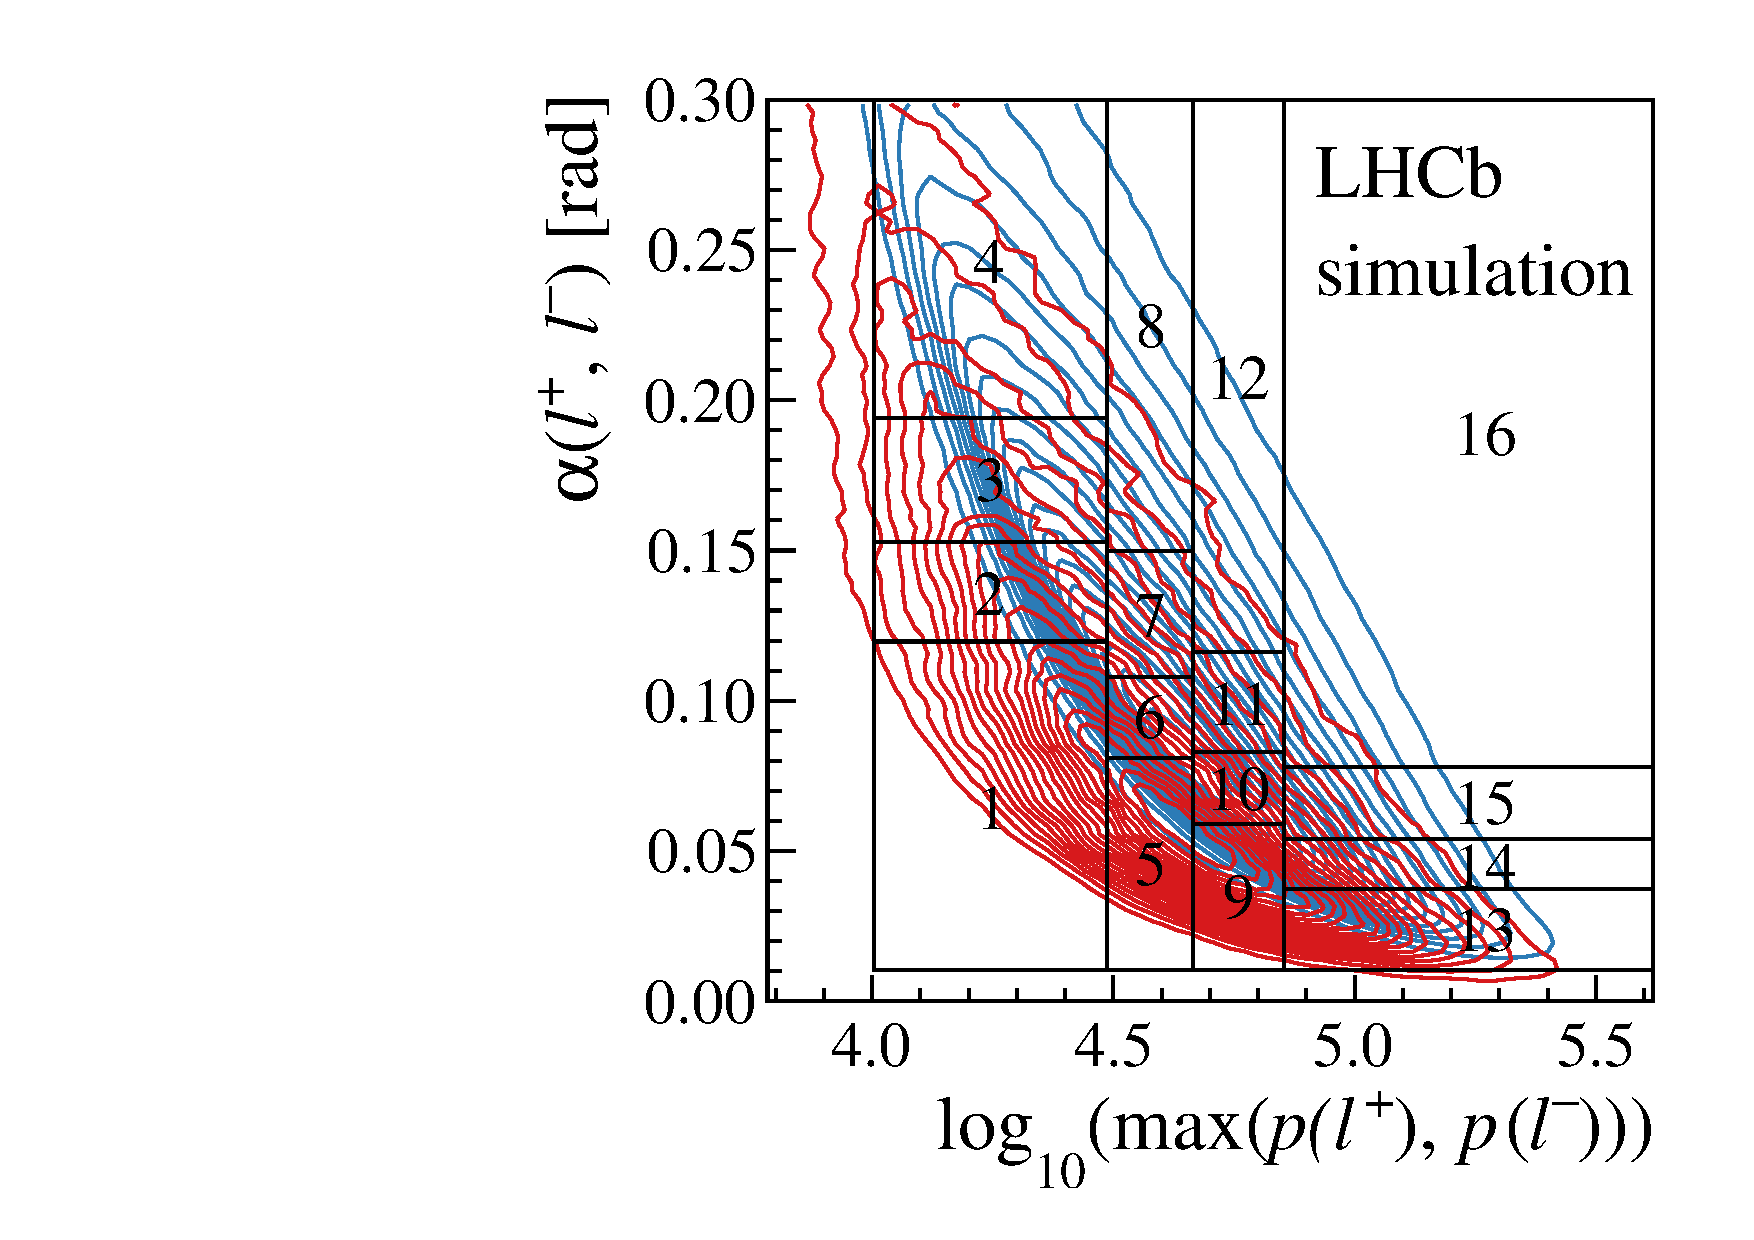
\includegraphics[height=0.32\linewidth]{figures/Fig10b.pdf}
   \end{center}
     \caption{Double differential \rjpsi measurement. (Left) the value of \rjpsi, relative to the average value of \rjpsi, measured in two-dimensional bins of the maximum lepton momentum, $p(l)$, and the opening angle between the two leptons, $\alpha(l^+,l^-)$. (Right) the bin definition in this two-dimensional space together with the
     distribution for \BuKee (\BuJpsiKee) decays depicted as red (blue) contours.}
    \label{fig:rjpsi_bin}
\end{figure}




\subsubsection*{Systematic uncertainties}

The majority of the sources of systematic uncertainty affect the relative efficiencies between nonresonant and resonant decays. These are included in the fit to \RK by allowing the relative efficiency to vary within Gaussian constraints. The width of the constraint is determined by adding the contributions from the different sources in quadrature. Correlations in the systematic uncertainties between different trigger categories and run periods are taken into account. Systematic uncertainties affecting the determination of the signal yield are assessed using pseudoexperiments generated with variations of the fit model. Pseudoexperiments are also used to assess the degree of bias originating from the fitting procedure. The bias is found to be 1\% of the statistical precision, \ie negligible with respect to other sources of systematic uncertainty.

For the nonresonant \BuKee decays, the systematic uncertainties are dominated by the modelling of the signal and background components used in the fit. The effect is at the 1\% level. A significant proportion (0.7\%) of this  uncertainty comes from the limited knowledge of the $K\pi$ spectrum in \BuBdKpiplusee decays. In addition, a 0.2\% systematic uncertainty is assigned for the potential contribution from \BuBdKpipiplusee events. 
A comparable uncertainty to that from the modelling of the signal and background components is induced by the limited sizes of calibration samples. Other sources of systematic uncertainty, such as the calibration of \Bu production kinematics, the trigger calibration and the determination of the particle identification efficiencies, contribute at the few-permille or permille level, depending strongly on the data-taking period and the trigger category. 


% The effect on \RK is at the $\pm0.008$ level. A  comparable uncertainty arises from the limited size of the calibration samples, with negligible contributions from the calibration of \Bu production kinematics and modelling of the selection and particle identification efficiencies. 

The uncertainties on parameters used in the simulation model of the signal decays affect the \qsq distribution and hence the selection efficiency. These uncertainties are propagated to an uncertainty on \RK using predictions from the {\sc{flavio}} software package~\cite{Straub:2018kue} but give rise to a negligible effect. Similarly, the differing \qsq resolution between data and simulation, which alters estimates of the \qsq migration, has negligible impact on the result.
